\documentclass[12pt]{article}

\usepackage[toc,page]{appendix}
\usepackage[spanish,es-tabla]{babel}
\usepackage[utf8]{inputenc}
\usepackage{amsmath}
\usepackage{amssymb}
\usepackage{array}
\usepackage{fancyhdr}
\usepackage{float}
\usepackage{graphicx}
\usepackage{hyperref}
\usepackage{listings}
\usepackage{longtable}
\usepackage{pdfpages}
\usepackage{textcomp}
\usepackage{xcolor}
\hypersetup{
    colorlinks=true,
    linkcolor=blue,
    filecolor=magenta,
    urlcolor=blue,
}
\lstset{
    language=Python,
    basicstyle=\ttfamily\small,
    keywordstyle=\color{blue},
    commentstyle=\color{green!50!black},
    stringstyle=\color{red},
    showstringspaces=false,
    breaklines=true,
    frame=single,
    numberstyle=\tiny,
    tabsize=4
}

\pagestyle{headings}
\textwidth=6.5in
\graphicspath{ {images/} }

% Define subsubsubsection
\setcounter{secnumdepth}{4}
\setcounter{tocdepth}{4}
\makeatletter
\newcounter{subsubsubsection}[subsubsection]
\renewcommand\thesubsubsubsection{%
    \thesubsubsection.\arabic{subsubsubsection}}
\newcommand\subsubsubsection[1]{%
    \par\refstepcounter{subsubsubsection}%
    \addcontentsline{toc}{paragraph}{\thesubsubsubsection\quad #1}%
    \noindent\textbf{\thesubsubsubsection\quad #1}\par
    \nobreak\smallskip
}
\makeatother

% ------------------------------------------------------------
\begin{document}
% ------------------------------------------------------------

\newcommand{\jhead}{Proyecto integrador}

\topmargin=-.5in
\oddsidemargin=.001in
\evensidemargin=.001in
\textheight=9in
\textwidth=6.5in

\pagestyle{fancy}

\fancyhead[L]{\protect\small \jhead}
\fancyhead[R]{\protect\small AD4036.10}

\fancypagestyle{firstpage}{%
 \lhead{\protect\small \jhead}
 \rhead{\protect\small TC5035.10}
}


% ============================================================
% PORTADA
% ============================================================

\begin{titlepage}

\centering

\vspace{1.5cm}

{
\includegraphics[width=0.50\textwidth]{tc_logo.png}\par}

\vfill

{\scshape\Large
Clasificación morfológica de galaxias mediante fusión multimodal de imágenes DESI Legacy y espectros integrados MaNGA
\par}

\vspace{1cm}

{\itshape\Large Proyecto Integrador \par}

\vspace{1cm}

{\large
\textbf{Presenta:}\par
Alexander Carreño (A01796955)\par
María Rabelero (A01793031)\par
Julio Ricardo Velázquez (A01796953)\par
}

\vspace{0.8cm}

{\large
\textbf{Equipo 26: Galaxy Vision}
\par}

\vfill

{\large
\textbf{Sponsor:}\par
Dr. José Antonio Vázquez Mata\par
Dr. Hector Manuel Hernandez Toledo\par
Instituto de Astronomía, UNAM
\par}

\vspace{0.8cm}

{\large
\textbf{Profesor:}\par
Dra. Grettel Barceló Alonso
\par}

\vfill

{\large México, 16 de septiembre de 2026 \par}

\end{titlepage}


\newpage

% ============================================================
% ÍNDICE
% ============================================================

\newpage

\tableofcontents

\newpage

% ============================================================
% 1. DATOS GENERALES DEL PROYECTO
% ============================================================

\section{Datos generales del proyecto}

% ------------------------------------------------------------
\subsection{Empresa / Institución}
% ------------------------------------------------------------

El beneficiario es el Instituto de Astronomía de la Universidad Nacional Autónoma de México (IA-UNAM), entidad pública de investigación dedicada a la investigación astronómica y astrofísica, a la formación de recursos humanos especializados y a la operación de infraestructura observacional nacional. El instituto participa de forma activa en colaboraciones internacionales de gran escala, entre ellas el APO (Apache Point Observatory) en Nuevo México, con el cual desarrollaron el programa de observación MaNGA (\textit{Mapping Nearby Galaxies at Apache Point}).

Dentro del instituto el beneficiario es el grupo de investigación en Galaxias y Cosmología. Este es responsable del \textit{Visual Morphology Value Added Catalogue} del MaNGA, un catálogo público de clasificación morfológica visual de 10,059 galaxias que incorpora imágenes de Hubble para la detección de rasgos y clasificación de galaxias. Este catálogo es la fuente de etiquetas del proyecto y la fuente de datos que este proyecto busca ampliar.

% ------------------------------------------------------------
\subsection{Sector Industrial}
% ------------------------------------------------------------

\begin{table}[H]
\centering
\small
\begin{tabular}{|p{0.20\textwidth}|p{0.12\textwidth}|p{0.57\textwidth}|}
\hline
\textbf{Nivel} & \textbf{Clave} & \textbf{Denominación} \\ \hline

Sector &
54 &
Servicios profesionales, científicos y técnicos \\ \hline

Rama / Subrama &
5417 &
Servicios de investigación científica y desarrollo \\ \hline

Clase de actividad &
541712 &
Servicios de investigación científica y desarrollo en ciencias naturales y exactas, ingeniería, y ciencias de la vida, prestados por el sector público.

\begin{itemize}
    \item Observatorios astronómicos, servicios del sector público.
\end{itemize}
\\ \hline

\end{tabular}
\caption{Sector Industrial}
\label{sector-industrial}
\end{table}

% ------------------------------------------------------------
\subsection{Lugar de Aplicación}
% ------------------------------------------------------------

\begin{table}[H]
\centering
\small
\begin{tabular}{|p{0.30\textwidth}|p{0.60\textwidth}|}
\hline

\textbf{País} &
México \\ \hline

\textbf{Estado} &
Ciudad de México \\ \hline

\textbf{Ciudad} &
Alcaldía Coyoacán \\ \hline

\textbf{Domicilio} &
Instituto de Astronomía, UNAM. Circuito Exterior s/n, Ciudad Universitaria, C.P. 04510 \\ \hline

\textbf{Área / Departamento / División} &
Área de investigación en Galaxias y Cosmología \\ \hline

\end{tabular}
\caption{Lugar de Aplicación}
\label{aplicacion}
\end{table}

% ------------------------------------------------------------
\subsection{Patrocinador o Sponsor}
% ------------------------------------------------------------

% Sponsor 1 --------------------------------------------------

\begin{table}[H]
\centering
\small
\begin{tabular}{|p{0.27\textwidth}|p{0.63\textwidth}|}
\hline

\textbf{Nombre} &
Dr. José Antonio Vázquez Mata \\ \hline

\textbf{Cargo} &
\begin{minipage}[t]{\linewidth}
\begin{itemize}
    \item Investigador posdoctoral, Instituto de Astronomía, UNAM (programa Estancias Posdoctorales por México).
    \item Profesor de asignatura en la Facultad de Ciencias, UNAM.
\end{itemize}
\end{minipage}
\\ \hline

\textbf{Adscripción} &
Instituto de Astronomía, UNAM Ciudad Universitaria, CDMX \\ \hline

\textbf{Correo institucional} &
\href{mailto:jvazquez@astro.unam.mx}{jvazquez@astro.unam.mx} \\ \hline

\textbf{Formación} &
Doctorado en Astronomía por la University of Sussex, Reino Unido \\ \hline

\textbf{Área de investigación} &
Galaxias y Cosmología; especialidad en astronomía óptica \\ \hline

\textbf{Reconocimientos} &
Sistema Nacional de Investigadoras e Investigadores \\ \hline

\end{tabular}
\end{table}

% Sponsor 2 --------------------------------------------------

\begin{table}[H]
\centering
\small
\begin{tabular}{|p{0.27\textwidth}|p{0.63\textwidth}|}
\hline

\textbf{Nombre} &
Dr. Hector Manuel Hernandez Toledo \\ \hline

\textbf{Cargo} &
\begin{minipage}[t]{\linewidth}
\begin{itemize}
    \item Investigador titular de tiempo completo, Instituto de Astronomía, UNAM
    \item Profesor de asignatura en la Facultad de Ciencias, UNAM
\end{itemize}
\end{minipage}
\\ \hline

\textbf{Adscripción} &
Instituto de Astronomía, UNAM Ciudad Universitaria, CDMX \\ \hline

\textbf{Correo institucional} &
\href{mailto:hector@astro.unam.mx}{hector@astro.unam.mx} \\ \hline

\textbf{Formación} &
Doctorado en Astrofísica por la UNAM, con tesis doctoral en la Universidad de Alabama, EUA \\ \hline

\textbf{Área de investigación} &
Astrofísica extragaláctica y cosmología observacional \\ \hline

\textbf{Reconocimientos} &
Sistema Nacional de Investigadores Nivel II, disciplina Astronomía Óptica \\ \hline

\end{tabular}
\caption{Sponsors}
\label{Sponsors}
\end{table}

Los sponsor son autores de varios artículos de investigación sobre clasificación morfológica de galaxias y de formación estelar usando \textit{machine learning}. También son los autores del catálogo de etiquetas con el cual trabajaremos en este proyecto. Esto reduce dos de los riesgos críticos del CRISP-ML porque ambos convergen en las mismas personas.

\begin{itemize}
    \item Separación de los expertos de dominio y los científicos de datos.
    \item Definición de los objetivos de ML y los objetivos de negocio.
\end{itemize}

En sus roles como sponsors del proyecto:

\begin{itemize}
    \item Nos darán acceso e interpretación de los datos del catálogo morfológico de espectros MaNGA, y de las imágenes del catálogo DESI Legacy Imaging Survey, el cual cuenta con la mejor base óptica para clasificar morfología de galaxias en el hemisferio norte.
    \item Validarán el éxito y aceptación del modelo.
    \item Actuarán como experto en la fase de evaluación.
\end{itemize}

% ------------------------------------------------------------
\subsection{Dominio de aplicación}
% ------------------------------------------------------------

El enfoque de IA es modelos predictivos con aprendizaje supervisado.

El problema se formula como clasificación supervisada. El objetivo es aprender una función capaz de replicar el criterio experto en galaxias no vistas, que produce una probabilidad calibrada. El aprendizaje supervisado es el enfoque correcto por dos razones:

\begin{itemize}
    \item El criterio a aprender es un criterio humano basado en conocimientos especializados que sólo puede transferirse por ejemplos.
    \item Lo que se necesita como salida es una decisión bajo incertidumbre discreta, no un agrupamiento.
\end{itemize}

% ------------------------------------------------------------
\subsubsection{Estrategia}
% ------------------------------------------------------------

Planeamos usar visión por computador, redes convolucionales sobre recortes de imagen de DESI Legacy Imaging Survey, que extraen la estructura, resolución de brazos y grado de inclinamiento.

También se plantea aplicar redes convolucionales o \textit{transformers} sobre el espectro y los ajustes de los espectros, ya que los tipos tardíos son más jóvenes, azules, ricos en formación estelar y pobres en metales que los tempranos, y esas diferencias quedan impresas en el espectro.

% ------------------------------------------------------------
\subsection{Plan de entregables}
% ------------------------------------------------------------

Los siguientes entregables son de referencia del curso y una guía para nuestro proyecto, siguen el calendario de 11 semanas de la materia. Los entregables comprometidos para el proyecto solo son cuatro: Planteamiento del proyecto, Avance 6: Producto de difusión, Avance 7: Resumen ejecutivo, y Presentación final.

\small

\begin{longtable}{|>{\raggedright\arraybackslash}p{0.05\textwidth}|>{\raggedright\arraybackslash}p{0.22\textwidth}|>{\raggedright\arraybackslash}p{0.50\textwidth}|>{\raggedright\arraybackslash}p{0.18\textwidth}|} \hline
\textbf{Sem.} & \textbf{Entregable} & \textbf{Qué se espera} & \textbf{Comprometido} \\ \hline \endfirsthead
\hline
\textbf{Sem.} & \textbf{Entregable} & \textbf{Qué se espera} & \textbf{Comprometido} \\ \hline \endhead

1 &
Planteamiento del proyecto &
Este documento. Propuesta, problemática del sector y de la institución, objetivos general y específicos, casos de uso de ML, metodología CRISP-ML, título, institución beneficiaria, lugar de aplicación, sponsor, dominio y enfoque de IA, y plan de entregables. &
Sí
\\ \hline

3 &
Avance 1: Análisis exploratorio de datos &
Notebook con el análisis de los datos, cuantificación de valores faltantes e inspección visual de espectros e imágenes de ejemplo por clase, verificación de calidad de datos, riesgos y esquema de datos. &
No
\\ \hline

4 &
Avance 2: Ingeniería de características &
Pipeline de preparación, construcción de las etiquetas, limpieza, corrección y remuestreo de espectros, normalización, recorte y ajuste de zoom de imágenes, y cálculo de características tabulares derivadas. Conjuntos de entrenamiento, validación y prueba. &
No
\\ \hline

5 &
Avance 3: Baseline &
Modelos entrenados y evaluados, con métricas, matriz de confusión y análisis de importancia de características. Documentado y reproducible que establece el piso de desempeño obligatorio. &
No
\\ \hline

6 &
Avance 4: Modelos alternativos &
Modelos de \textit{deep learning} monomodal (sólo imagen, sólo espectro y sólo ajuste de espectro) y multimodal, evaluados bajo el mismo protocolo, con costos computacionales y comparados contra el baseline. &
No
\\ \hline

7 &
Avance 5: Modelo final &
Modelo multimodal de fusión, ablación cuantificando la ganancia atribuible a la fusión, análisis de calibración y desempeño desagregado por inclinación, masa estelar, corrimiento al rojo y bandera de galaxia tenue, difusa, compacta. El modelo seleccionado se justificará y validará. &
No
\\ \hline

8 &
Avance 6: Producto de difusión &
Documentación del proyecto y sus resultados, ejemplos de aciertos y errores, y explicación de la contribución multimodal. Material autocontenido dirigido a un público sin conocimiento previo de \textit{machine learning}. &
Sí
\\ \hline

9 &
Avance 7: Resumen ejecutivo &
Versión final del documento con los resultados del proyecto, con conclusiones y dirigido a un tomador de decisiones, incluye recomendaciones sobre las mejores aplicaciones en el sector. &
Sí
\\ \hline

10--11 &
Presentación final &
Exposición de la solución implementada ante asesor y sponsor, con sesión de preguntas y respuestas. &
Sí
\\ \hline

\caption{Entregables}
\label{Entregables}
\end{longtable}

\normalsize

% ------------------------------------------------------------
\subsection{Repositorio del proyecto}
% ------------------------------------------------------------

\begin{itemize}
    \item \url{https://github.com/AlexanderCarreno/clasificacion-galaxias}
\end{itemize}

% ============================================================
% 2. PLANTEAMIENTO
% ============================================================

% ------------------------------------------------------------
\section{Planteamiento del Proyecto Integrado}
\subsection{Antecedentes}
\subsubsection{Instituto de Astronomía de la UNAM}
% ------------------------------------------------------------

El Instituto de Astronomía de la Universidad Nacional Autónoma de México (IA-UNAM) es la institución encargada de la investigación en astronomía y astrofísica dentro de la UNAM, así como del resguardo, mantenimiento y operación del Observatorio Astronómico Nacional (OAN). Está integrado por dos sedes académicas en Ciudad Universitaria, en la Ciudad de México, y en Ensenada, Baja California.

Su misión es desarrollar la astrofísica en México a través de la investigación, la enseñanza y el desarrollo de instrumentación astronómica. El Instituto cuenta con una planta de más de 80 investigadores y un número similar de técnicos académicos, y desde 2012 la UNAM forma parte de la colaboración Sloan Digital Sky Survey (SDSS).

El es responsable del \textit{Visual Morphology Value Added Catalogue} del sondeo MaNGA (parte de SDSS-IV), un catálogo público de clasificación morfológica visual de 10,059 galaxias que incorpora imágenes de Hubble para la detección de rasgos y clasificación de galaxias. Este catálogo es la fuente de etiquetas del proyecto y la fuente de datos que este proyecto busca ampliar.

Esto es relevante para este proyecto ya que los espectros que usaremos han sido analizados por el instituto lo que garantiza acceso, experiencia previa y continuidad científica sobre los datos que usaremos.

% ------------------------------------------------------------
\subsubsection{Clasificación Morfológica de Galaxias}
% ------------------------------------------------------------

La morfología de una galaxia es uno de los descriptores más antiguos y más informativos de la historia de formación estelar y el ambiente en que la galaxia evolucionó. El tipo morfológico describe la forma y la estructura visible de las galaxias. Las galaxias se ordenan mediante sus rasgos como la concentración de estrellas en su centro, la presencia de disco y el grado de apertura de los brazos espirales mediante la secuencia de Hubble.

\begin{figure}[H]
    \centering
    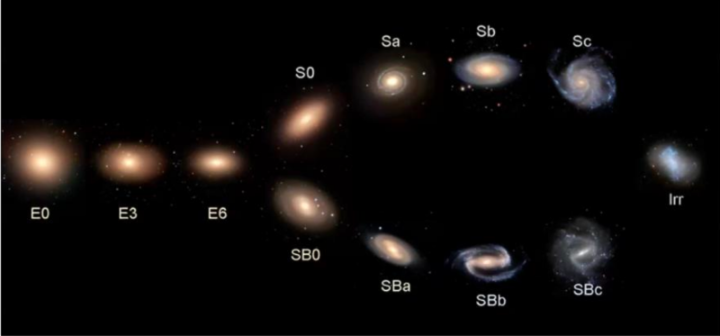
\includegraphics[width=0.70\textwidth]{tipos_galaxias.png}
    \caption{Secuencia de Hubble. Elípticas (E0--E6), Espirales normales y barradas (S0--Sc y SB0--SBc), Irregulares (Irr).}
    \label{fig:Escala-Ttype}
\end{figure}

La secuencia de Hubble separa sistemas de galaxias tempranas (\textit{early-type} ETG) de sistemas tardías (\textit{late-type}, LTG), y que se resume numéricamente mediante el índice T-Type.

\begin{figure}[H]
    \centering
    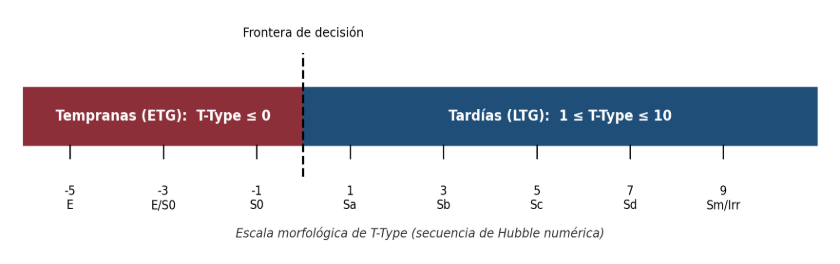
\includegraphics[width=0.70\textwidth]{escala_ttype.png}
    \caption{Esquema de índice T-Type. Las galaxias con T-Type $\leq$ 0 se etiquetan como tempranas (ETG) y las que cumplen 1 $\leq$ T-Type $\leq$ 10 como tardías (LTG)}
    \label{fig:hubble}
\end{figure}

% ------------------------------------------------------------
\subsubsection{ Proceso Impactado: Clasificación de Galaxias }
% ------------------------------------------------------------

El proceso impactado es la generación y uso de catálogos de clasificación morfológica. Actualmente el proceso de la clasificación morfológica se realiza de forma visual. Un experto observa la imagen de la galaxia y decide el tipo morfológico. La clasificación visual es útil pero incorpora incertidumbre y depende de la profundidad, resolución, orientación, longitud de onda y relación señal-ruido de la imagen. También afecta la inclinación, el polvo y la banda de observación que pueden afectar la apariencia de estructuras.

Hasta el momento no existe un trabajo que combine espectros e imágenes con fines de clasificación morfológica. La literatura de \textit{machine learning} en el tema es abundante pero solo están basadas en imágenes. Lo que no existe al momento es un trabajo que combine espectros e imágenes. Ahí se sitúa la contribución del proyecto.

% ------------------------------------------------------------
\subsection{Entendimiento del Negocio}
\subsubsection{Formulación del problema}
% ------------------------------------------------------------

Los sondeos producen catálogos de cientos de millones a miles de millones de objetos, y el método predominante de clasificación morfológica sigue siendo la inspección visual, lo que plantea limitaciones:

\begin{itemize}
    \item La clasificación depende de cuán abiertos o cerrados se perciban los brazos espirales. En el MaNGA cerca del 10 \% tienen clasificación dudosa por su aspecto tenue, difuso o compacto, y 67 objetos resultaron inclasificables.
    \item El tiempo de integración del telescopio y el brillo superficial límite de la cámara impiden capturar la estructura en los extremos de los brazos y las estructuras de bajo brillo superficial, lo que sesga sistemáticamente la clasificación hacia tipos más tempranos.
    \item Los catálogos morfológicos derivados de imágenes tipo Hubble contienen entre 20–30 mil galaxias clasificadas, y los catálogos de ciencia ciudadana alcanzan aproximadamente medio millón. Frente al volumen de los cartografiados actuales y futuros, la clasificación visual no es sostenible.
\end{itemize}

La necesidad de un cambio se vuelve crítica ante la llegada de una nueva generación de instrumentos. En junio de 2026, el Observatorio Vera C. Rubin inició el Legacy Survey of Space and Time (LSST), un sondeo de diez años que cartografiará el cielo austral con una cámara de 3,200 megapíxeles y generará aproximadamente 10 terabytes de datos por noche.

A lo largo del sondeo, cada región del cielo será observada unas 800 veces. La combinación de todas estas observaciones permitirá obtener imágenes más profundas y nítidas, detectar galaxias más débiles y mejorar sustancialmente su clasificación morfológica.

\begin{figure}[H]
    \centering
    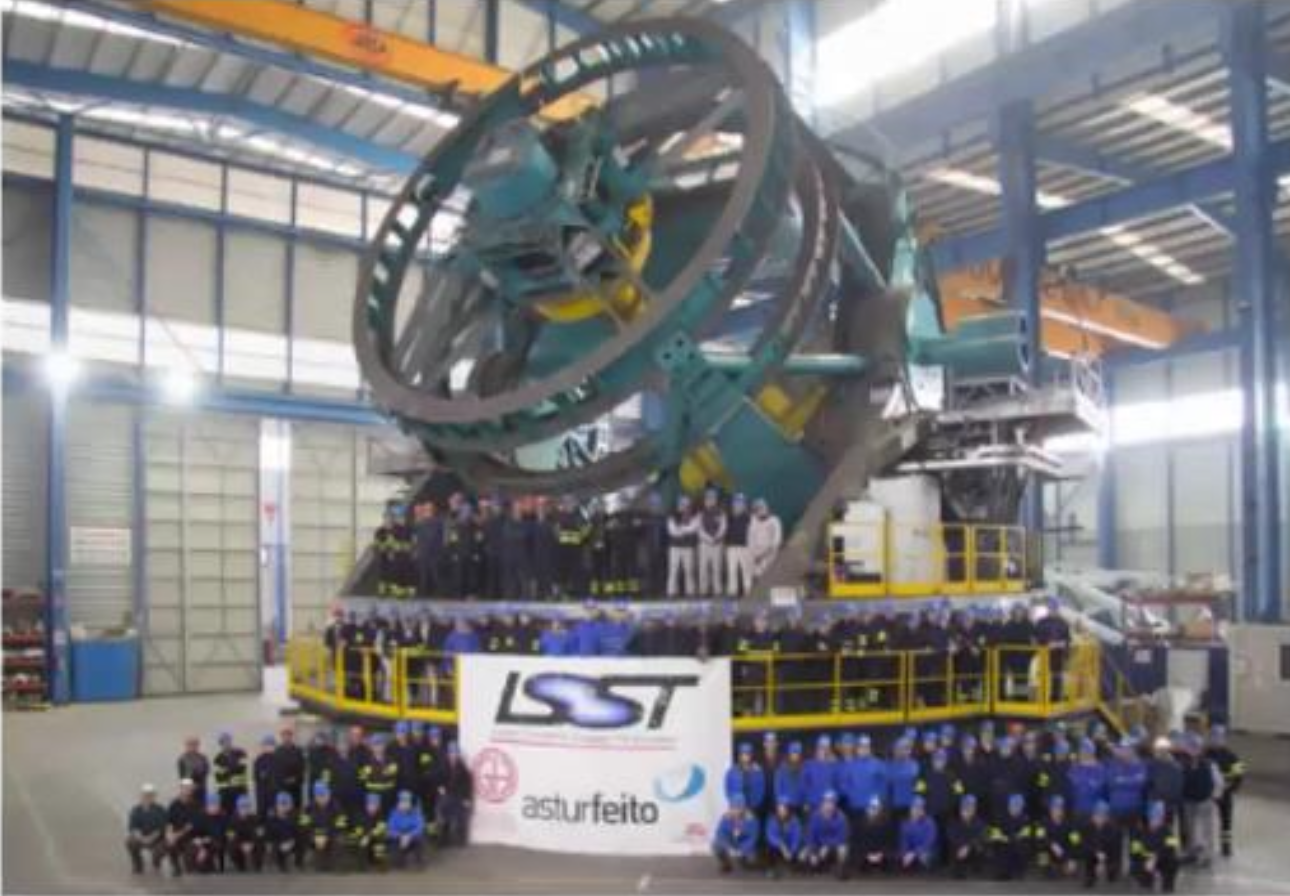
\includegraphics[width=0.62\textwidth]{telescopio.png}
    \caption{El Observatorio Vera C. Rubin, su sondeo LSST redefine la escala del problema.}
    \label{fig:rubin}
\end{figure}

El Instituto, a través del APO, ha invertido un esfuerzo humano considerable en clasificar visualmente las galaxias del MaNGA. Sin embargo, replicar este procedimiento para los millones de galaxias que observará LSST resulta materialmente imposible. La institución necesita transformar ese capital intelectual en un clasificador automático.

% ------------------------------------------------------------
\subsubsection{Contexto}
% ------------------------------------------------------------

\begin{itemize}
    \item \textbf{Escala:} La inspección manual no crece al ritmo de los cartografiados astronómicos y de los futuros, que producirán mayor cantidad y profundidad.
    \item \textbf{Reproducción:} Un modelo versionado aplica reglas consistentes y poder repetir el mismo resultado con los mismos datos.
    \item \textbf{Complementar:} La imagen aporta la estructura espacial (grado de apertura de los brazos espirales), el espectro aporta la composición física (edad, metalicidad, tasa de formación estelar, contenido de gas ionizado), usar ambas para poder clasificarlas según la secuencia de Hubble.
\end{itemize}

% ------------------------------------------------------------
\subsection{Objetivos}
\subsubsection{Objetivo General}
% ------------------------------------------------------------

Desarrollar y evaluar un clasificador morfológico de galaxias que integre imágenes del DESI Legacy Imaging Surveys y espectros de MaNGA, comparando arquitecturas de \textit{deep learning}, con el fin de determinar cuál constituye la mejor aplicación para el sector astronómico ante el volumen de datos de la nueva generación de sondeos.

% ------------------------------------------------------------
\subsubsection{Objetivos Específicos}
% ------------------------------------------------------------

\begin{itemize}
    \item Realizar un análisis exploratorio de la distribución de T-Type, balance entre clases tempranas y tardías, cobertura de \textit{redshift}, masa estelar, inclinación y tamaño angular, e identificar los casos en los que existe mayor incertidumbre en las etiquetas.
    \item Definir y ejecutar la ingeniería de características: normalización del espectro, remuestreo de longitud de onda, y ajuste del zoom del recorte de imagen para homogeneizar el tamaño de las galaxias.
    \item Definir un modelo de referencia para establecer el umbral mínimo de desempeño (\textit{baseline}) para las arquitecturas subsecuentes.
    \item Entrenar y comparar modelos unimodales (sólo imagen, sólo espectro, solo ajuste de espectros) y multimodales (fusión de \textit{embeddings}), evaluar cuánto mejora el desempeño gracias a la fusión de modalidades.
    \item Evaluar los modelos en términos de exactitud, calibración, costo computacional y esfuerzo de ajuste de hiperparámetros.
    \item Analizar los errores de la inclinación, masa estelar, clasificación de galaxia, para definir las condiciones bajo las cuales el modelo produce resultados fiables.
    \item Presentar una recomendación sobre la adopción del enfoque en el sector astronómico, junto con un modelo de difusión y un resumen ejecutivo para la toma de decisiones.
\end{itemize}

% ------------------------------------------------------------
\subsubsection{Preguntas Clave}
% ------------------------------------------------------------

\begin{itemize}
    \item ¿La combinación de imagen y espectro mejora de forma significativa la clasificación respecto a usar únicamente imágenes o únicamente espectros o únicamente ajuste de espectros?
    \item ¿Cuánta información morfológica contiene realmente un espectro y sus resultados de ajuste espectral, medida como desempeño de un clasificador que sólo lo utiliza?
    \item ¿Qué regiones del espectro y de su ajuste espectral (población estelar, líneas de emisión, forma del continuo) resultan más útiles para separar tempranas de tardías?
    \item ¿Un modelo fundacional tabular alcanza un desempeño competitivo frente a las redes profundas, con menor costo de entrenamiento y menos datos etiquetados?
    \item ¿Cómo se comporta el clasificador en la zona de transición -1 < T-Type < 2, y qué porcentaje de casos requieren revisión humana?
    \item ¿Es transferible el modelo a imágenes de mayor profundidad, como las que producirá el nuevo telescopio por empalme de exposiciones?
\end{itemize}

% ------------------------------------------------------------
\subsubsection{Involucrados}
% ------------------------------------------------------------

En el proyecto participan varios grupos: el grupo científico del IA-UNAM que aporta el dominio y la validación, el equipo de estudiantes que construye los modelos; y los académicos, cuya participación es supervisar el proyecto.

\begin{table}[H]
\centering
\scriptsize
\begin{tabular}{|p{0.22\textwidth}|p{0.22\textwidth}|p{0.22\textwidth}|p{0.22\textwidth}|} \hline
\textbf{Participante} & \textbf{Etapa de participación} & \textbf{Tipo de involucramiento} & \textbf{Nivel} \\ \hline

Investigadores en evolución de galaxias, IA-UNAM  &
Antecedentes, entendimiento del negocio y validación de resultados  &
Definición del problema científico, criterios morfológicos, interpretación astrofísica de los resultados  &
Alto, patrocinador científico y validador final
\\ \hline

Estudiantes de posgrado, ITESM &
Preparación de datos, construcción de modelos y experimentación  &
Descarga y control de calidad de imágenes, experimentos de ajuste de hiperparámetros  &
Medio, participación operativa
\\ \hline

Cuerpo académico, ITESM  &
Hitos y liberación  &
Recepción de la metodología &
Revisa la metodología, riesgos, resultados y condiciones de aceptación
\\ \hline

\end{tabular}
\caption{Matriz de Involucrados}
\label{involucrados}
\end{table}


% ------------------------------------------------------------
\subsection{Entendimiento de los Datos}
\subsubsection{Descripción de los datos de entrada}
% ------------------------------------------------------------

El conjunto de datos del proyecto es multimodal. Cada galaxia es descrita simultáneamente por una imagen, un espectro, un ajuste espectral y por un conjunto de atributos tabulares, todos ellos vinculados mediante el identificador de la galaxia en el catalogo MaNGA. Las modalidades provienen de fuentes distintas y fueron producidas con propósitos distintos y con un control de calidad distinto.

Los principales datos que utilizaremos provienen de imágenes de galaxias. Las descargaremos del catálogo DESI Legacy Imaging Surveys en formato \texttt{.fits}. Estas sólo se pueden bajar por cada banda (canal) \texttt{grz}. Se usarán las imágenes en su escala natural, adecuando el zoom de las galaxias para tener una mejor clasificación, mediante el radio aproximado de la galaxia (\texttt{PETRO\_TH90}). Con este se pretende variar la escala que es el valor que modifica el zoom.

Las galaxias que usaremos provienen de un archivo compartido por el sponsor \texttt{morfologia.fits}, el cual contiene 10,127 registros con nueve columnas:

\begin{itemize}
    \item \texttt{name}: Identificador MaNGA.
    \item \texttt{objra} y \texttt{objdec}: Ascensión recta y declinación en grados.
    \item \texttt{Type}: Tipo de Hubble, variantes barradas SB/SAB y S-merger.
    \item \texttt{Ttype}: Tipo de convención.
    \item \texttt{nsa\_z}: \textit{Redshift} del NASA-Sloan Atlas.
    \item \texttt{LogMass}: Logaritmo de la masa estelar.
    \item \texttt{incl}: Inclinación en grados.
    \item \texttt{PETRO\_TH90}: Radio petrosiano.
\end{itemize}

También se compartió un archivo ZIP MPL-11 con 10,127 archivos de formato \texttt{.fits} con información de los espectros. Cada archivo contiene cinco columnas:

\begin{itemize}
    \item \texttt{WAVE}: Longitud de onda. Se usa para generar el espectro y se remuestrea a una malla común para que cada posición del vector signifique lo mismo en todas las galaxias.
    \item \texttt{flux\_1re}: Radio Efectivo. Resume la energía observada dentro de campo observado. Es el portador de la señal espectral, el continuo espectral y las líneas de emisión y absorción reflejan la población estelar y la actividad de formación estelar que covarían con la morfología.
    \item \texttt{flux\_fov}: Campo Visual. Espectro integrado sobre todo el campo de visión del instrumento. Provee las mismas carecteriricas que el radio eefectivo.
    \item \texttt{error\_1re}: Indice de error de la metrica \texttt{flux\_1re}.
    \item \texttt{error\_fov}: Indice de error de la metrica \texttt{flux\_1re}.
\end{itemize}

De igual manera, también se compartió un archivo ZIP FoV-OUT con 10,127 archivos de texto de extensión \texttt{.out}. Estos son los resultados del ajuste de los espectros anteriores usando el programa STARLIGHT. Se construyo un espectro modelo usando componentes de un espectro y la combinación de poblaciones estelares, su polvo y su movimiento, ajustando todo a un modelo base que se estima mejor reproduce la luz de la galaxia. La sección principal del archivo contiene una fila por cada componente del modelo, que normalmente es una población con una edad y una metalicidad dadas, de él salen las edades medias, las metalicidades medias y la historia de formación estelar. Y quince columnas:

\begin{itemize}
    \item \texttt{j}: Índice del componente. Identifica a qué modelo corresponde la fila.
    \item \texttt{x\_j(\%)}: Contribución de luz del componente en la longitud de onda de normalización \texttt{l\_norm}. Se expresa porcentualmente respecto a la escala de normalización del ajuste.
    \item \texttt{Mini\_j(\%)}:Fracción de la masa estelar inicial, contando la masa que se devolvió al medio interestelar por evolución estelar.
    \item \texttt{Mcor\_j(\%)}: Fracción de la masa estelar actual, ya descontada la masa devuelta al medio interestelar por supernovas y vientos.
    \item \texttt{age\_j(yr)}: Edad del componente en años. Es una propiedad del modelo base, no una edad ajustada continuamente.
    \item \texttt{Z\_j}: Metalicidad. La fracción de masa en elementos más pesados que el helio, con \texttt{Z = 0.02}.
    \item \texttt{(L/M)\_j}: Valor del espectro en la longitud de onda de normalización, conservando las unidades originales de la base. P.
    \item \texttt{YAV?}: Indicador de extinción. Indicador (0 o 1) de si el componente puede tener la extinción extra.
    \item \texttt{Mstars}: Fracción de la masa inicial que permanece en estrellas a la edad del componente. Se utiliza para convertir contribuciones de luz en fracciones de masa actual.
    \item \texttt{component\_j}: identificador del componente tomado del archivo maestro de la base.
    \item \texttt{a\/Fe}: Relación de abundancia del componente.
    \item \texttt{SSP\_chi2r}: Es el chi-cuadrado dividido entre el número de píxeles utilizados de ese ajuste con un solo componente.
    \item \texttt{SSP\_adev(\%)}: Desviación relativa media porcentual de ese ajuste con un solo componente.
    \item \texttt{SSP\_AV}: Extinción \texttt{AVA\_VAV} en magnitudes, de ese ajuste con un solo componente.
    \item \texttt{SSP\_x(\%)}: Factor de normalización equivalente a \texttt{sum-of-x} de ese ajuste con un solo componente.
\end{itemize}

% ------------------------------------------------------------
\subsubsection{Descripción de los datos de salida}
% ------------------------------------------------------------

La salida del modelo sera el T-Type de las galaxias, mediante una regla: y = 0 para tempranas cuando T-Type $\leq$ 0; y = 1 para tardías cuando 1 $\leq$ T-Type $\leq$ 10. Deben excluirse o marcarse para revisión los valores faltantes, no numéricos o fuera del dominio acordado. La codificación debe conservar también T-Type original para auditoría y análisis de errores cerca de la frontera 0/1.

\begin{table}[H]
\centering
\scriptsize
\begin{tabular}{|p{0.22\textwidth}|p{0.22\textwidth}|p{0.12\textwidth}|p{0.32\textwidth}|} \hline
\textbf{Condición en T-Type} & \textbf{Clase} & \textbf{Código} & \textbf{Tratamiento} \\ \hline

T-Type $\leq$  0 &
Temprana &
0 &
Incluir si cumple controles de calidad. \\ \hline

1 $\leq$ Ttype $\leq$ 10 &
Tardía &
1 &
Incluir si cumple controles de calidad. \\ \hline

Faltante o fuera del rango definido &
No asignada &
NA &
No usar para entrenamiento supervisado; revisar por separado. \\ \hline

\end{tabular}
\caption{Regla de construcción de la etiqueta}
\label{etiquetas}
\end{table}

% ------------------------------------------------------------
\subsubsection{Técnica de ML}
% ------------------------------------------------------------

La técnica es aprendizaje supervisado de clasificación binaria, resuelto con aprendizaje profundo multimodal.

\begin{itemize}
    \item \texttt{Supervisado:} Cada galaxia tiene una etiqueta conocida, Ttype, que asignaron expertos. El modelo aprende de pares (datos, etiqueta).
    \item \texttt{Clasificación:} T-Type se convierte en dos clases: \textbf{temprana} (0) si T-Type $\leq$  0 y \textbf{tardía} (1) si 1 $\leq$  T-Type $\leq$  10. No se predice el valor continuo de T-Type.
    \item \texttt{Profundo}: Todos los modelos son redes neuronales entrenadas de extremo a extremo:

        \begin{itemize}
            \item \texttt{Imágenes:} Una CNN de 4 bloques y una ResNet-18.
            \item \texttt{Espectros:} CNN1D, CNN con atención, CNN + BiGRU y Patch + BiGRU.
            \item \texttt{Poblaciones STARLIGHT:} Una red MLP.
            \item \texttt{Fusión:} Concatenación de las ramas y, como siguiente fase, un mecanismo de gating/stacking que decida cuánto confiar en cada modelo por galaxia.
        \end{itemize}

\end{itemize}

A continuación se presentan las familias de modelos evaluados en los experimentos efectuados.

\small

\begin{longtable}{|>{\raggedright\arraybackslash}p{0.22\textwidth}|>{\raggedright\arraybackslash}p{0.12\textwidth}|>{\raggedright\arraybackslash}p{0.32\textwidth}|>{\raggedright\arraybackslash}p{0.22\textwidth}|}
\hline \textbf{Experimento} & \textbf{Familia} & \textbf{Configuración} & \textbf{Por qué se incluye} \\ \hline \endfirsthead
\hline \textbf{Experimento} & \textbf{Familia} & \textbf{Configuración} & \textbf{Por qué se incluye} \\ \hline \endhead

Binario solo imágenes con opción GPU &
CNN 2D compacta &
Red convolucional pequeña, entrenada desde cero. Aprende de lo simple (bordes, texturas) a lo complejo (bulbo, disco, brazos) y resume la imagen en un vector con el que decide temprana o tardía. Con versión GPU.  &
Modelo baseline, comprueba que el pipeline funciona y que un modelo barato aprende la morfología. Entrenar más épocas no mejoró. \\ \hline

Binario imágenes con FOV aleatorio y GPU &
CNN 2D compacta  &
La misma CNN, pero en cada paso de entrenamiento la galaxia aparece con un zoom distinto (FOV \textminus1, 0 o \textpm1, según \texttt{PETRO\_TH90)}. Funciona como aumento de datos. &
Evalúa si variar el encuadre ayuda a generalizar y reduce el sobreajuste. \\ \hline

ResNet-18 solo imágenes &
CNN residual  &
Red más profunda con atajos que facilitan el aprendizaje. Se configuró exactamente como la rama visual de las fusiones y mismas reglas de entrenamiento.  &
Es un control, si una fusión mejora se sabe que fue por el dato añadido y no por cambiar de red. \\ \hline

Espectros FoV, solo espectros &
CNN 1D &
Filtros que recorren el espectro buscando patrones locales (línea de emisión a 4000Å) y luego lo promedian. Una máscara que ignora las zonas sin datos.  &
Referencia espectroscópica con datos observados, mide cuánta morfología hay en la luz. \\ \hline

Espectros STARLIGHT, solo los ajuste de los espectros &
CNN 1D &
La misma red aplicada al espectro modelado por STARLIGHT, que tiene menos ruido. &
Compara el espectro observado con el modelado. La diferencia fue mínima. \\ \hline

Espectros FoV, 3 variantes &
CNN 1D con atención, CNN + BiGRU, RNN (Patch + BiGRU) &
3 formas de leer mejor el espectro: atención (aprende qué zonas pesan más), CNN + BiGRU (resume tramos y los relaciona a lo largo del espectro) y Patch + BiGRU (lee el espectro como una secuencia de trozos). &
La CNN 1D no aprovechaba bien el espectro (subajuste). La variante con atención es el control sin recurrencia. \\ \hline

Espectros STARLIGHT, 3 variantes &
CNN 1D con atención, CNN + BiGRU, RNN (Patch + BiGRU) &
Las mismas tres arquitecturas, aplicadas al espectro STARLIGHT. &
Verifica si la mejora se repite con el espectro modelado. La atención basta y la recurrencia no aporta. \\ \hline

Poblaciones STARLIGHT, Solo poblaciones STARLIGHT &
Perceptrón multicapa (MLP) &
Red densa sencilla para 90 números tabulares (proporciones de estrellas por edad y metalicidad), normalizados y regularizados. &
Aporta contexto físico interpretable y barato. Fue el dato no visual más fuerte de la ablación. \\ \hline

Multimodal de poblaciones STARLIGHT, espectro y poblaciones STARLIGHT &
Fusión por concatenación (CNN 1D + MLP) &
Cada dato pasa por su experto; los resúmenes se unen y una red final decide. &
Comprueba si espectro y poblaciones se complementan sin la imagen. No hubo mejora (0.896 frente a 0.895), porque ambos salen del mismo ajuste. \\ \hline

Multimodal de imagenes y espectros FoV &
Fusión por concatenación (ResNet-18 + CNN 1D) &
Une el resumen de la imagen con el del espectro y decide con una red final. Todo se entrena junto. &
Es la hipótesis original del proyecto: imagen + espectro FoV. AUC igual que la imagen sola. \\ \hline

Multimodal de imagenes y espectros STARLIGHT &
Fusión por concatenación (CNN 2D compacta + CNN 1D con atención) &
Combina los dos mejores expertos individuales. Incluye un control de solo imagen con la misma red y el mismo entrenamiento, que difiere solo en no recibir el espectro. &
Un experto espectral no mejora la fusión. La fusión cayó frente a la imagen sola. \\ \hline

Multimodal de imagenes y poblaciones STARLIGHT &
Fusión por concatenación (ResNet-18 + MLP) &
Une la estructura visual con el contexto físico. &
Las poblaciones fueron el dato más complementario. Sin mejora demostrable. \\ \hline

Multimodal de imagenes, espectros y poblaciones STARLIGHT &
Fusión por concatenación (ResNet-18 + CNN 1D + MLP) &
3 expertos (imagen, espectro, poblaciones). Sus resúmenes se unen y una red final decide. &
Prueba si combinar todo da el máximo. Fue el mejor multimodelo, pero solo una diferencia minima sobre la imagen sola. \\ \hline

\caption{Familias de modelos que se evaluaron}
\label{modelos}
\end{longtable}

\normalsize


A continuación se muestra la arquitectura del mejor multimodelo.

\begin{figure}[H]
    \centering
    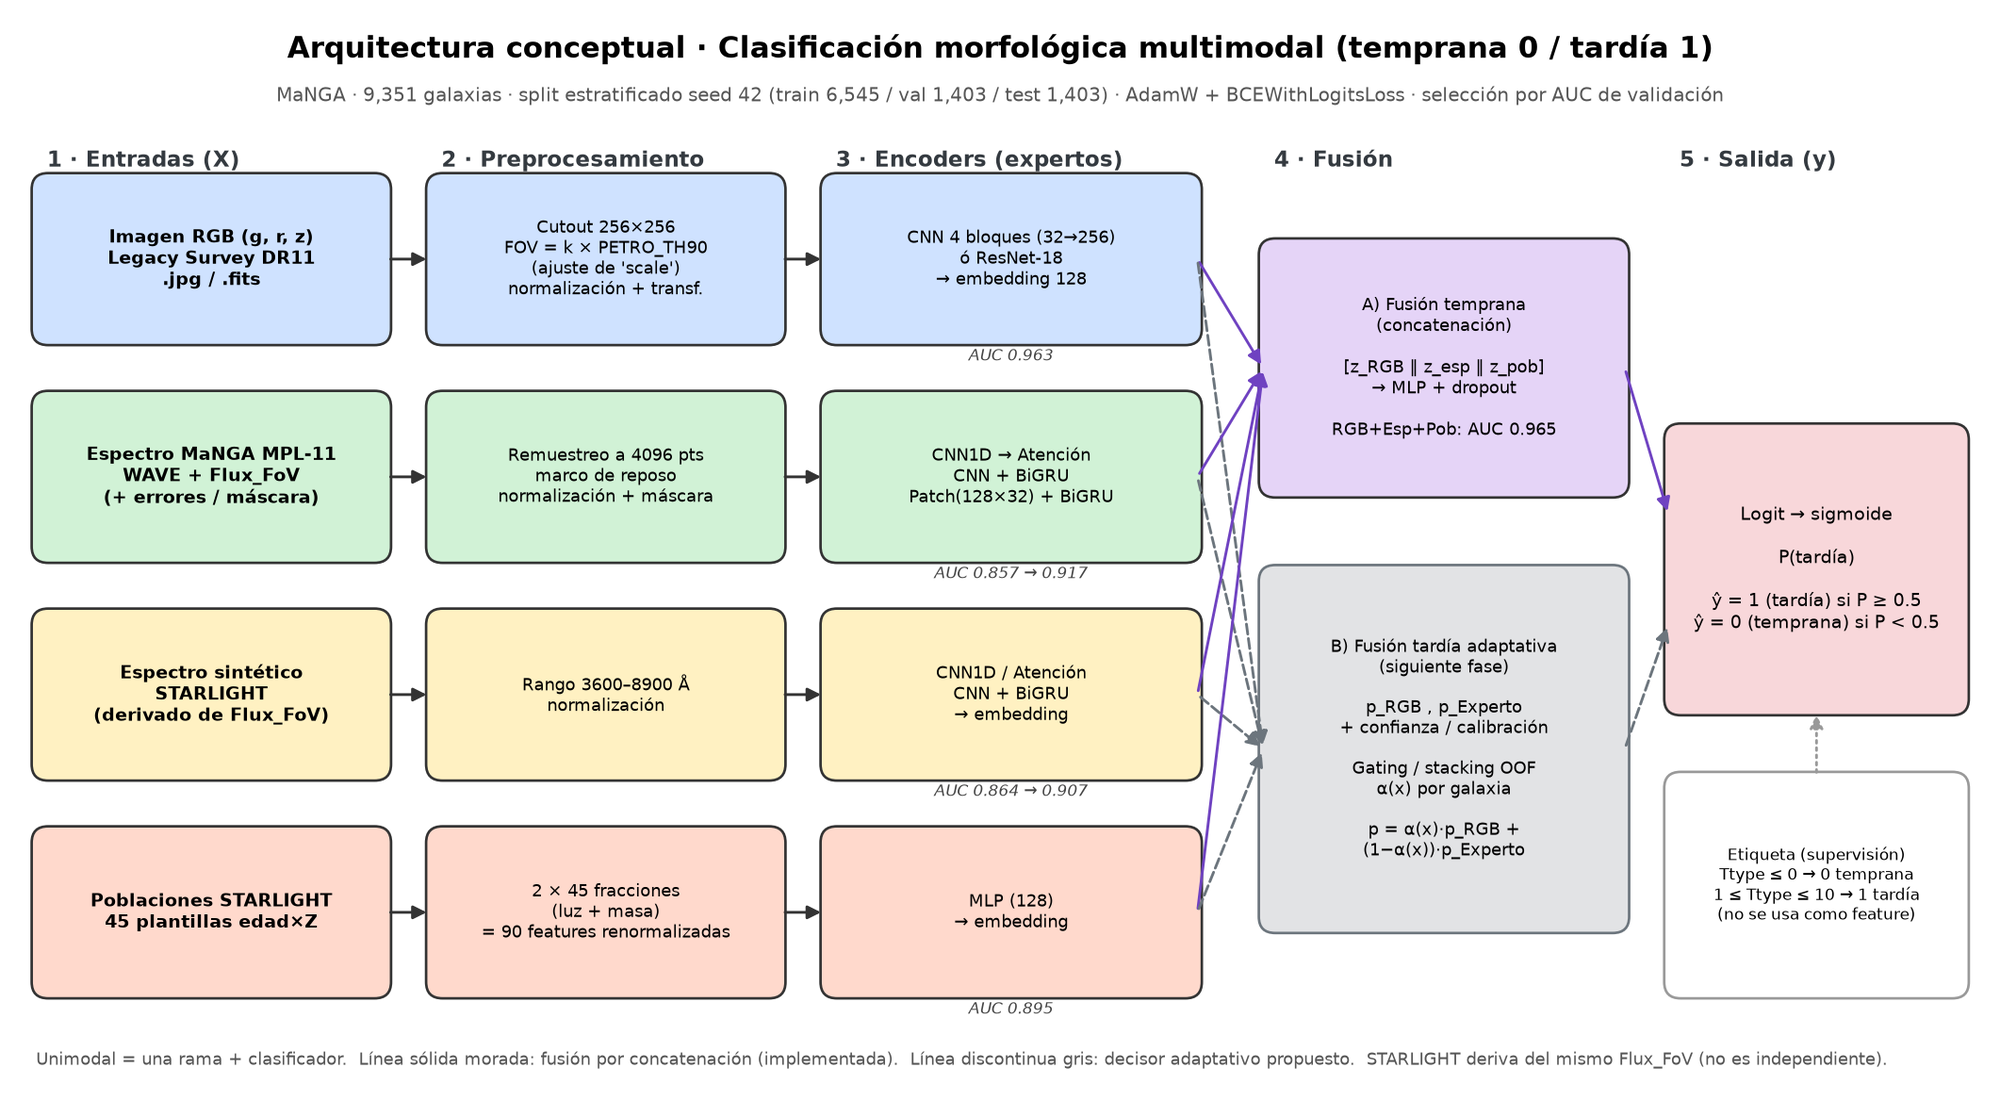
\includegraphics[width=0.62\textwidth]{modelos.png}
    \caption{Arquitectura conceptual del clasificador multimodal. Cada modalidad se procesa en una rama independiente y sus representaciones se fusionan antes de la decisión final.}
    \label{fig:modelos}
\end{figure}


% ------------------------------------------------------------
\subsection{Metodología}
% ------------------------------------------------------------

El proyecto se desarrolla siguiendo CRISP-ML(Q) (\textit{Cross-Industry Standard Process model for the development of Machine Learning applications with Quality assurance methodology}), el cual combina entendimiento del negocio y de los datos en una sola fase e introduce en cada tarea la identificación de riesgos y el método de calidad que los mitiga.

Este proyecto solo cubre las primeras cuatro fases; despliegue y monitoreo quedan documentados como trabajo futuro.

\begin{figure}[H]
    \centering
    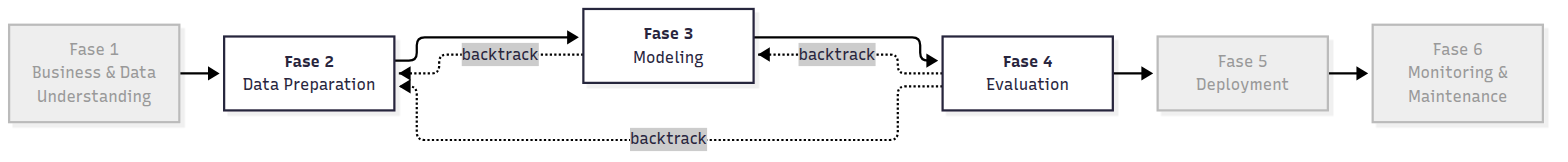
\includegraphics[width=0.65\textwidth]{diag2_fases.png}
    \caption{Encadenamiento de las fases.}
    \label{fig:crisp}
\end{figure}

% ------------------------------------------------------------
\subsubsection{Fase 1: Entendimiento del negocio y de los datos}
% ------------------------------------------------------------

\begin{itemize}
    \item \textbf{Alcance}
    El proyecto busca desarrollar y evaluar un sistema de inteligencia artificial para la clasificación morfológica binaria de galaxias tempranas y tardías, combinando imágenes y espectros integrados. Se plantea que ambas fuentes contienen información complementaria y que su combinación podría producir una clasificación más fiable que el uso de una sola modalidad.

    Se compararán modelos de \textit{machine learning} tanto por su capacidad predictiva como por su utilidad para aplicaciones en el sector astronómico.
    \item \textbf{Criterios de éxito en tres niveles}

    \begin{itemize}
        \item \textbf{Negocio:}
        Obtener una clasificación científicamente útil y determinar si la combinación de imágenes y espectros integrados aporta valor.
        \item \textbf{ML:}
        Alcanzar un rendimiento mínimo que sobrepase al trabajo anterior, \textit{Accuracy: 0.829} y \textit{F1-score: 83\%}. Los modelos deberán alcanzar sensibilidad adecuada en ambas clases y probabilidades fiables. Ningún modelo debe situarse por debajo de la línea base.
        \item \textbf{Económico (KPI):}
        Reducir el esfuerzo de clasificación y revisión, en términos de tiempo por galaxia, memoria y proporción de objetos que requieren revisión humana. Mientras se mantiene un costo computacional razonable.
    \end{itemize}

    \item \textbf{Factibilidad.}
    Revisando la literatura sobre la clasificación morfológica con \textit{machine learning} el tamaño muestral ($\sim$10 mil objetos etiquetados visualmente) resulta suficiente para un clasificador automático, y existen precedentes de \textit{CNN bayesianas} con alta exactitud usando solo imágenes. No hay restricciones legales o económicas ya que los datos son públicos y de acceso abierto.
    \item \textbf{Recolección de datos.}
    Los sponsors son los responsables de brindar el catálogo de trabajo, el equipo de estudiantes es el responsable de descargar las 10,127 imágenes de las galaxias del catálogo DESI Legacy Imaging Surveys.

    \begin{table}[H]
        \centering
        \scriptsize
        \begin{tabular}{|p{0.15\textwidth}|p{0.20\textwidth}|p{0.20\textwidth}|p{0.20\textwidth}|}
        \hline
        \textbf{Datos} & \textbf{Fuente} & \textbf{Contenido} & \textbf{Uso en el proyecto} \\
        \hline

        \textbf{Catálogo} &
        \texttt{morfologia.fits} &
        \texttt{name, objra, objdec, Type, Ttype, nsa\_z, LogMass, incl, PETRO\_TH90} &
        Etiquetas, llave de integración textit{name} y tamaño angular para el zoom. \\ \hline

        \textbf{Espectros} &
        \texttt{MaNGA MPL-11.zip} (manga-plate-ifu-1D.fits) &
        \texttt{WAVE, FLUX\_1RE, FLUX\_FoV, ERROR\_1RE, ERROR\_FoV} &
        Modalidad espectral. \\ \hline

        \textbf{STARLIGHT} &
        \texttt{Starlight FoV-OUT.zip} (manga-plate-ifu-1D.out) &
        Espectro modelado, 45 poblaciones (BC03) y propiedades derivadas. &
        Modalidad espectral modelada y \texttt{poblaciones estelares}.\\ \hline

        \textbf{Imágenes} &
        \texttt{legacysurvey.org} &
        Cutouts grz (DR11). &
        Modalidad visual\\ \hline

        \end{tabular}
        \caption{Fuentes de datos}
        \label{aplicacion}
    \end{table}

\end{itemize}

% ------------------------------------------------------------
\subsubsection{Fase 2: Preparación de los datos}
% ------------------------------------------------------------

Esta tarea comprende Feature selection, Data selection y Unbalanced Classes.

\textbf{Selección de datos}.

\begin{itemize}
    \item \textbf{Selección de características}

    \begin{table}[H]
        \centering
        \scriptsize
        \begin{tabular}{|p{0.40\textwidth}|p{0.40\textwidth}|} \hline
        \textbf{Características} & \textbf{Decisión} \\ \hline

        Imagen RGB grz &
        Entrada principal \\ \hline

        Espectro \texttt{FLUX\_FoV} &
        Modalidad espectro \\ \hline

        Poblaciones STARLIGHT (2×45=90 valores) &
        Modalidad derivada \\ \hline

        \texttt{nsa\_z, LogMass, PETRO\_TH90, final\_pixscale} &
        Solo en experimentos de contexto \\ \hline

        \texttt{label, Ttype, Type, name, objra, objdec} &
        Prohibidas como entrada \\ \hline

        \end{tabular}
        \caption{Feature Selection}
        \label{aplicacion}
    \end{table}

    \item \textbf{Selección de muestras}. Se unen todas las fuentes por la columna \textit{name}. Los cruces son uno a uno y nunca dependen del orden de los archivos. Resultado: 10,014 galaxias en el catálogo, 10,013 con FITS y 9,351 en la cohorte experimental.
    
    \begin{table}[H]
        \centering
        \scriptsize
        \begin{tabular}{|p{0.15\textwidth}|p{0.25\textwidth}|p{0.25\textwidth}|p{0.15\textwidth}|}
        \hline
        \textbf{Datos} & \textbf{Fuente} & \textbf{Criterio} & \textbf{Galaxias} \\
        \hline

        Catálogo curado &
        \texttt{morfologia\_curada.csv} &
        \textit{Type} dentro de las reglas, con \texttt{PETRO\_TH90} y coordenadas válidas &
        10,014 \\ \hline

        Imágenes &
        \texttt{legacysurvey.org} &
        Imagen no sospechosa en FOV \textpm1, 0, y \textminus1 &
        9,351 \\ \hline

        Espectros &
        MaNGA \texttt{MPL-11.zip} (manga-plate-ifu-1D.fits) &
        \textit{WAVE, FLUX\_1RE, FLUX\_FoV, ERROR\_1RE, ERROR\_FoV} &
        10,013 \\ \hline

        \end{tabular}
        \caption{División de clases}
        \label{aplicacion}
    \end{table}

    \item \textbf{Clases desbalanceadas}. El 62\% de la muestra son galaxias tardías. Por eso la partición es estratificada y la evaluación usa métricas que no premian a la clase mayoritaria. No se aplica remuestreo. Se mitiga con un split estratificado 70/15/15 (semilla 42) y un umbral elegido en validation. Resultando en:
    
    \begin{table}[H]
        \centering
        \scriptsize
        \begin{tabular}{|p{0.20\textwidth}|p{0.20\textwidth}|p{0.20\textwidth}|p{0.20\textwidth}|}
        \hline
        \textbf{Clase} & \textbf{Tardía} & \textbf{Temprana} & \textbf{Galaxias} \\
        \hline

        \textbf{Entrenamiento} &
        4,078 (62.3\%) &
        2,467 (37.7\%) &
        6,545 \\ \hline

        \textbf{Validación} &
        874 &
        529 &
        1,403 \\ \hline

        \textbf{Prueba} &
        875 &
        528 &
        1,403 \\ \hline

        \end{tabular}
        \caption{Clases en cada partición}
        \label{aplicacion}
    \end{table}

    \begin{figure}[H]
    \centering
    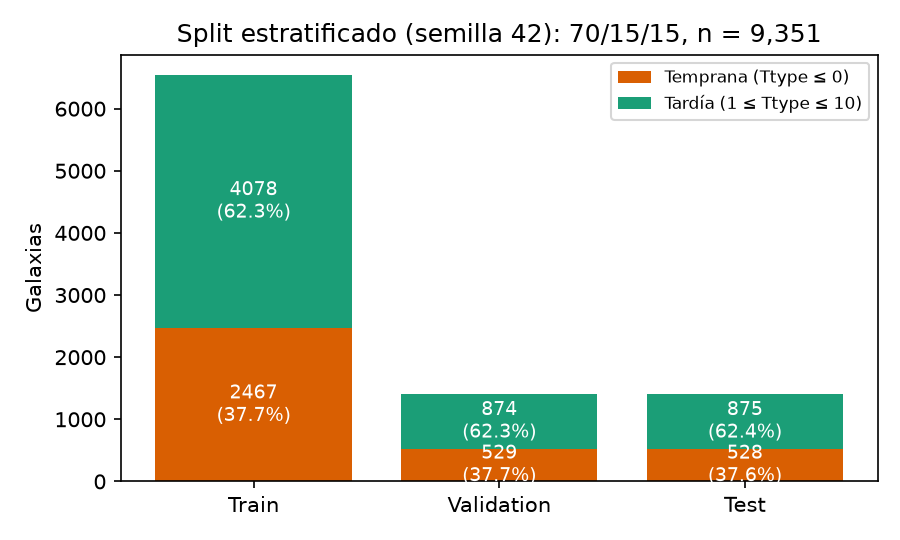
\includegraphics[width=0.65\textwidth]{fig1_split_clases.png}
    \caption{clases en cada partición (train/validation/test)}
    \label{fig:crisp}
    \end{figure}

\end{itemize}

\textbf{Limpieza de datos}.

\begin{itemize}
    \item \textbf{Reducción de ruido}. Se crea una máscara de color de la galaxia central para quitar estrellas de campo. Existen dos limitaciones: borra discos externos débiles y no separa galaxias vecinas. Cualquier filtro hay que evaluarlo comparándolo con la imagen original antes de adoptarlo. En la muestra de 1,000 galaxias, \textit{line\_flag} se activó en el 1.9\% de los casos.
    
    \begin{table}[H]
        \centering
        \scriptsize
        \begin{tabular}{|p{0.15\textwidth}|p{0.30\textwidth}|p{0.35\textwidth}|}
        \hline
        \textbf{Dato} & \textbf{Problema} & \textbf{Método} \\
        \hline

        \textbf{Imagen} &
        Líneas o artefactos de satélite, contaminación brillante, saturación &
        Detector heurístico: \textit{mapa\ max(R,G,B)}, z-score robusto (mediana\/MAD), perfiles por fila y columna, componentes conexos clasificados como \textit{is\_suspicious} \\ \hline

        \textbf{Imagen} &
        Estrellas de campo &
        Máscara de color (distancia de Mahalanobis entre galaxia y cielo) y la componente conexa central \\ \hline

        \textbf{Espectro} &
        NaN, valores fuera de rango, píxeles sin cobertura &
        Máscara de validez \texttt{spectrum\_mask} y pooling enmascarado \\ \hline

        \textbf{STARLIGHT} &
        Píxeles sin dato observado &
        Se escriben como NaN \\ \hline

        \end{tabular}
        \caption{Reducción de ruido}
        \label{aplicacion}
    \end{table}

    \item \textbf{Imputación}. No se imputan flujos espectrales. No se extrapola; los valores de relleno se ponen a 0 después de normalizar y la máscara impide que influyan. Los metadatos se imputan solo con estadísticas de train y llevan una máscara de ausencia.

\end{itemize}

\textbf{Construcción de datos}.

\begin{itemize}
    \item \textbf{Ingeniería de características}. 
    Se aplica un zoom adaptativo usando \textit{PETRO\_TH90}, con \textit{k} entre 4 y 8, el rango razonable resultó ser 5–8.

    \begin{figure}[H]
    \centering
    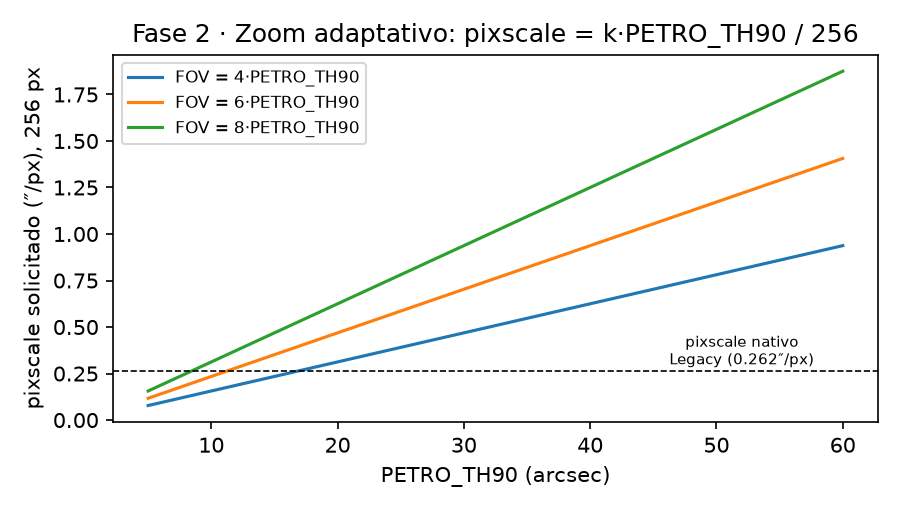
\includegraphics[width=0.65\textwidth]{fig5_fov_pixscale.png}
    \caption{Cómo cambia la escala de píxel según \textit{PETRO\_TH90}}
    \label{fig:crisp}
    \end{figure}

    Se aplica corrección del redshift a los espectros.

    \item \textbf{Aumento de datos}. Rotaciones de 0\textdegree, 90\textdegree, 180\textdegree y 270\textdegree y volteos horizontal y vertical, solo durante el entrenamiento. La morfología no cambia con la orientación.
\end{itemize}

\textbf{Estandarización}.

\begin{itemize}
    \item \textbf{Normalización}. Las estadísticas se calculan con el conjunto de entrenamiento y se aplican sin cambios a validación y prueba.

    \begin{table}[H]
        \centering
        \scriptsize
        \begin{tabular}{|p{0.20\textwidth}|p{0.15\textwidth}|p{0.15\textwidth}|p{0.15\textwidth}|}
        \hline
        \textbf{Partición} & \textbf{Tempranas} & \textbf{Tardías} & \textbf{Total} \\ \hline

        \textbf{Entrenamiento} &
        2,467 &
        4,078 &
        6,545 \\ \hline

        \textbf{Validación} &
        529 &
        874 &
        1,403 \\ \hline

        \textbf{Prueba} &
        528 &
        875 &
        1,403 \\ \hline

        \end{tabular}
        \caption{Conjunto de entrenamiento }
        \label{aplicacion}
    \end{table}

    \item \textbf{Salida de la fase}. Manifest, partición persistente, cachés versionadas e informe de exclusiones (10,014 → 9,351 galaxias, con el motivo de cada exclusión).
\end{itemize}

\textbf{QA}.

\begin{figure}[H]
    \centering
    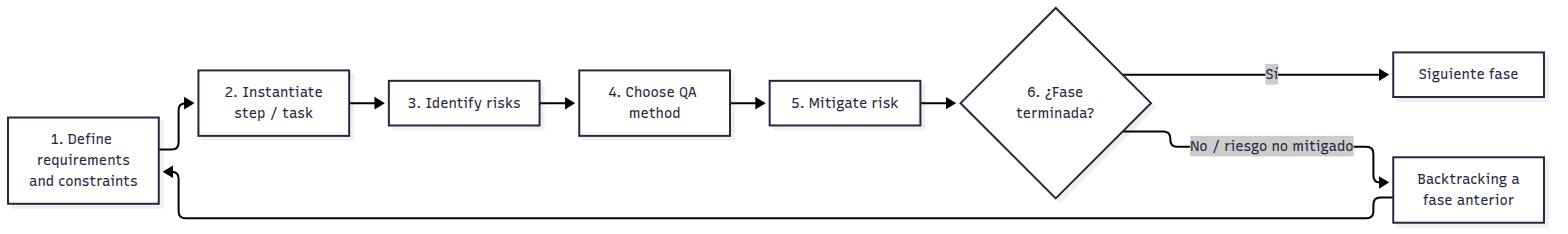
\includegraphics[width=0.65\textwidth]{diag1_ciclo_qa.png}
    \caption{Riesgos y QA de la fase 2}
    \label{fig:crisp}
\end{figure}

\textbf{Flujo de los datos}.

\begin{figure}[H]
    \centering
    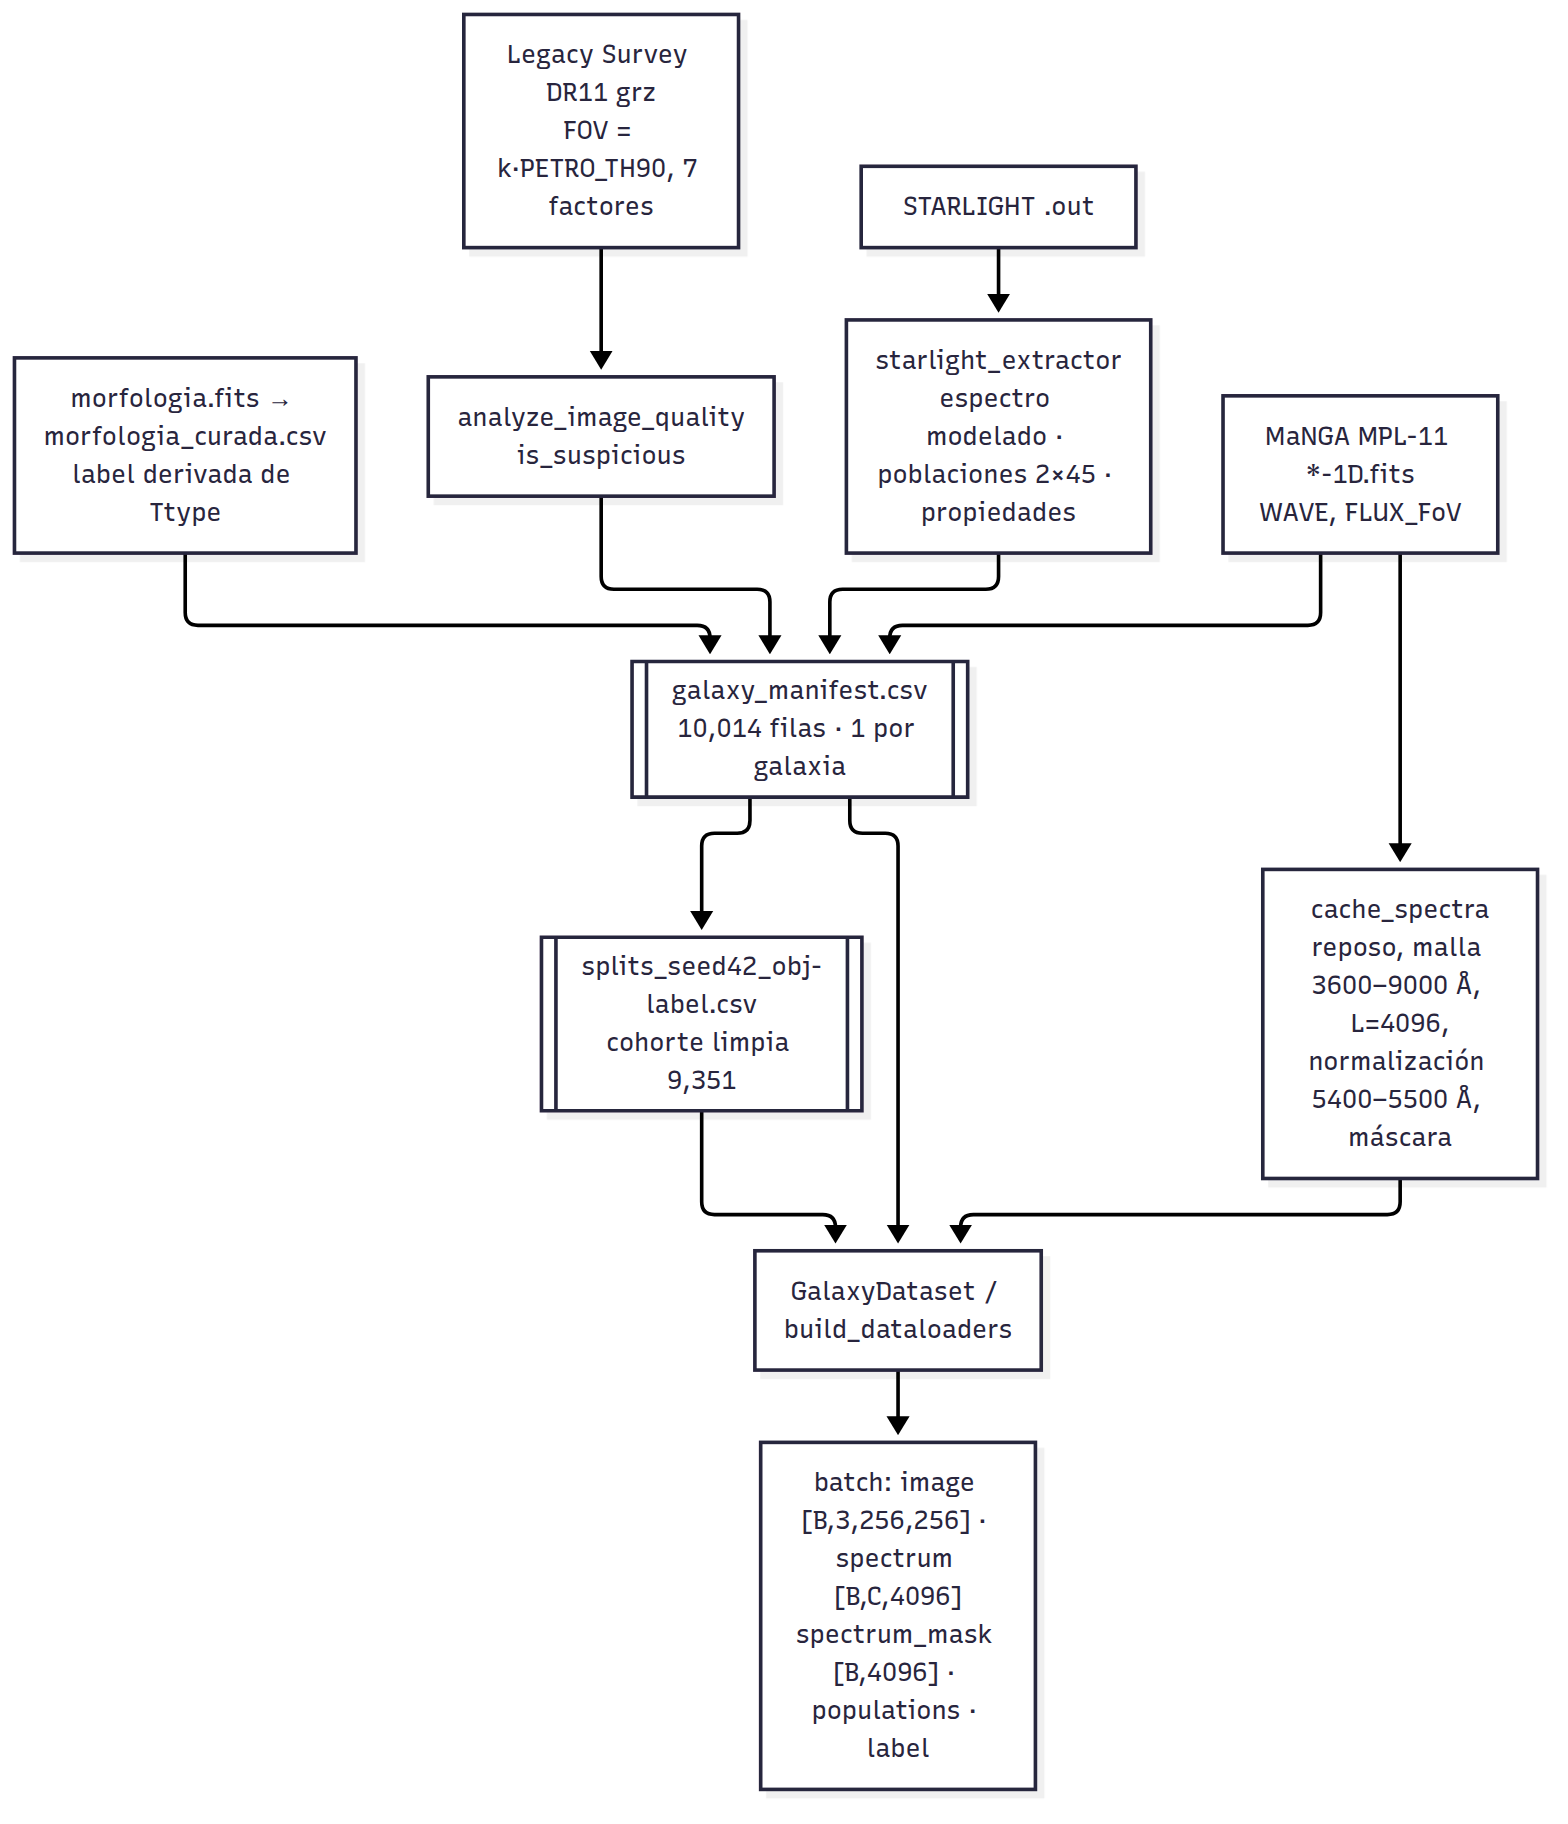
\includegraphics[width=0.65\textwidth]{diag3_flujo_datos.png}
    \caption{Flijo de datos}
    \label{fig:crisp}
\end{figure}

% ------------------------------------------------------------
\subsubsection{Fase 3: Modelado}
% ------------------------------------------------------------

Revisión de literatura y líneas base. Siguiendo la recomendación de empezar con modelos de poca capacidad e ir aumentándola, se hizo una ablación (comparar ramas por separado y en combinación).

\begin{figure}[H]
    \centering
    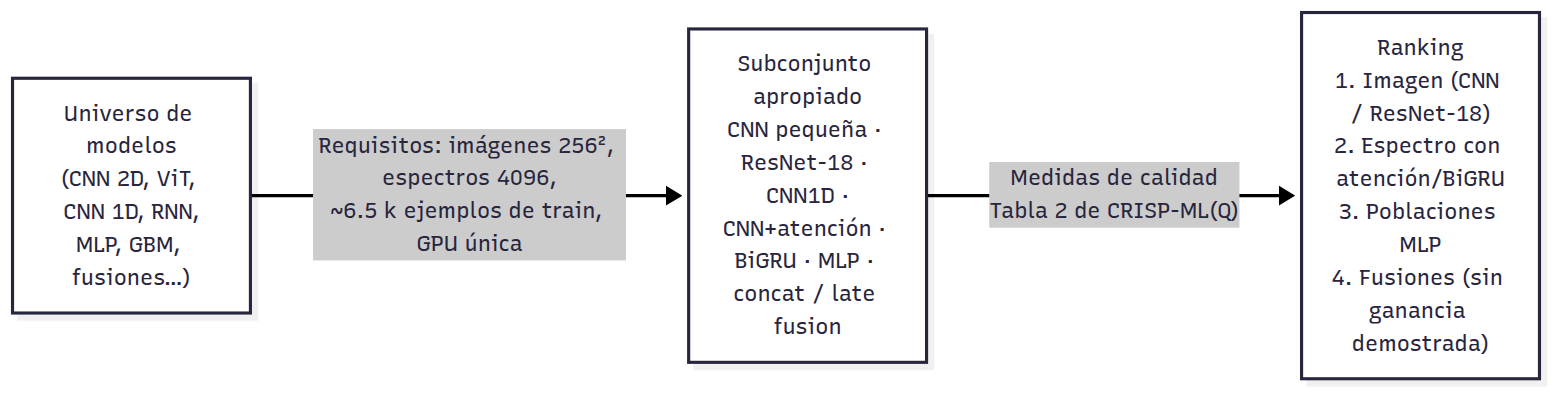
\includegraphics[width=0.65\textwidth]{diag4_seleccion_modelos.png}
    \caption{Modelado.}
    \label{fig:crisp}
\end{figure}

\textbf{Revisión de literatura}.

\begin{itemize}
    \item Se utilizo \texttt{Dieleman et al. (2015)} para la creacion de la CNN con invariancia a rotaciones (Galaxy Zoo).
    \item Se utilizo \texttt{Domínguez Sánchez et al. (2018; 2022)} como referencia en la muestra T-Type con CNN en SDSS/MaNGA.
    \item \texttt{Walmsley et al. (2022, Zoobot)} aporto los modelos preentrenados en Legacy Survey. 
    \item Se utilizo\texttt{Cid Fernandes et al. (2005)} Para el uso de la Base física de STARLIGHT.
\end{itemize}

\textbf{Medidas de calidad}.

\begin{table}[H]
    \centering
    \scriptsize
    \begin{tabular}{|p{0.40\textwidth}|p{0.40\textwidth}|}
    \hline
    \textbf{Medida} & \textbf{Definición} \\
    \hline

    \textbf{Performance} &
    \texttt{ROC-AUC, balanced accuracy, macro-F1, recall} por clase \\ \hline

    \textbf{Robustness} &
    Estabilidad ante FoV, semillas y ruido (FOV aleatorio, una sola semilla) \\ \hline

    \textbf{Scalability} &
    Tiempo por época \\ \hline

    \textbf{Explainability} &
    Plausibilidad física \\ \hline

    \textbf{Model Complexity} &
    Parámetros frente a datos (\texttt{CNN}$\approx1$.2M, \texttt{ResNet-18}$\approx$11M)\\ \hline

    \textbf{Resource Demand} &
    GPU única; $\sim$328MB de caché \\ \hline

    \end{tabular}
    \caption{Fuentes de datos}
    \label{aplicacion}
\end{table}

\textbf{Selección de modelos}.

\begin{table}[H]
    \centering
    \scriptsize
    \begin{tabular}{|p{0.25\textwidth}|p{0.30\textwidth}|p{0.25\textwidth}|}
    \hline
    \textbf{Modelo} & \textbf{Arquitectura} & \textbf{Experimento} \\ \hline

    Baseline visual (E1) &
    \texttt{CNN} de 4 bloques &
    \texttt{experimento\_binario\_imagenes\_cnn(\_gpu)} \\ \hline

    Control de capacidad &
    \texttt{ResNet-18} aleatorio &
    \texttt{imagenes\_resnet18\_fov} \\ \hline

    Baseline espectral (E2) &
    \texttt{CNN 1D} enmascarada &
    \texttt{espectros\_\{fov,starlight\}\_cnn1d} \\ \hline

    Baseline físico &
    \texttt{MLP} &
    \texttt{poblaciones\_starlight\_mlp} \\ \hline

    Fusión (E3) &
    Concatenación &
    \texttt{multimodal\_*\_concat} \\ \hline

    Espectro con más capacidad (E4) &
    Atención, \texttt{BiGRU} &
    \texttt{espectros\_*\_\{cnn\_attn\_control, cnn\_bigru, patch\_bigru\}} \\ \hline

    Fusión con espectro fuerte &
    \texttt{ResNet-18} + atención &
    \texttt{multimodal\_*\_cnnattn\_\{fusion, image\_only\_control\}} \\ \hline

    Aumentación de escala &
    \texttt{CNN} &
    \texttt{*\_fov\_aleatorio} \\ \hline

    \end{tabular}
    \caption{Conjunto de entrenamiento }
    \label{aplicacion}
\end{table}

\begin{figure}[H]
    \centering
    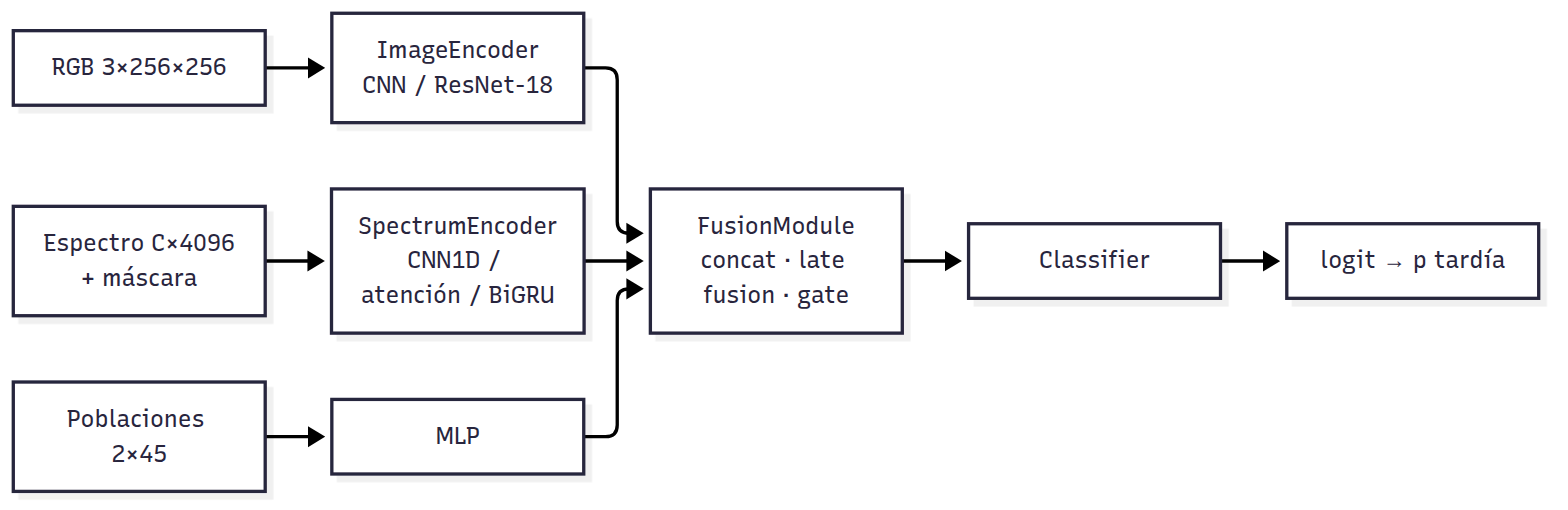
\includegraphics[width=0.65\textwidth]{diag5_arquitectura.png}
    \caption{Arquitectura multimodal.}
    \label{fig:crisp}
\end{figure}

\textbf{Conocimiento del dominio}. 

TBD

\textbf{Entrenamiento}. 

\begin{figure}[H]
    \centering
    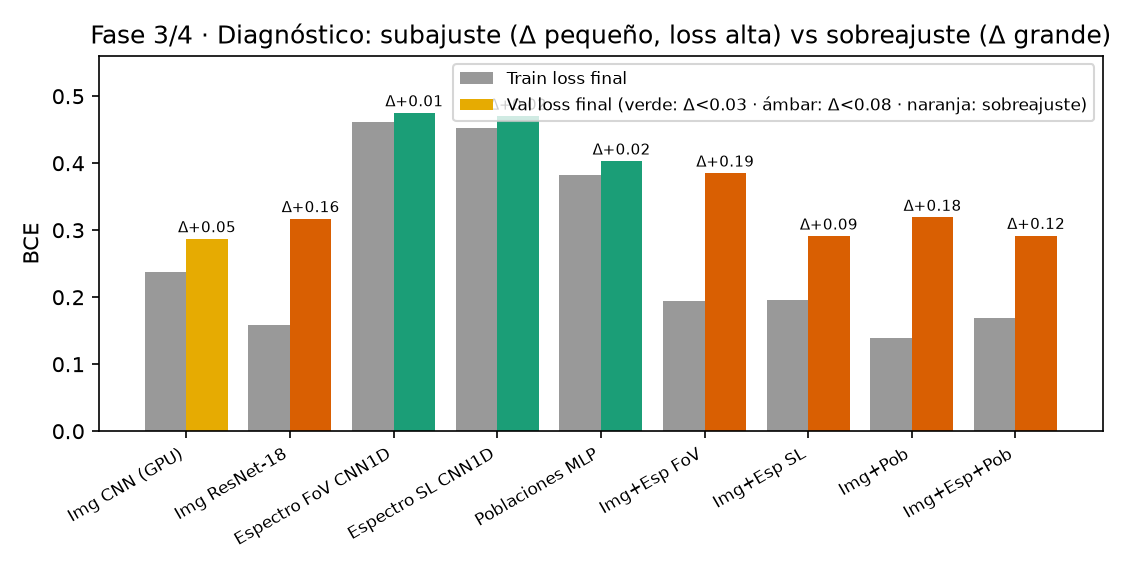
\includegraphics[width=0.65\textwidth]{fig4_brecha_train_val.png}
    \caption{Diferencia entre la pérdida de entrenamiento y la de validación, para ver sobreajuste o subajuste.}
    \label{fig:crisp}
\end{figure}

\begin{figure}[H]
    \centering
    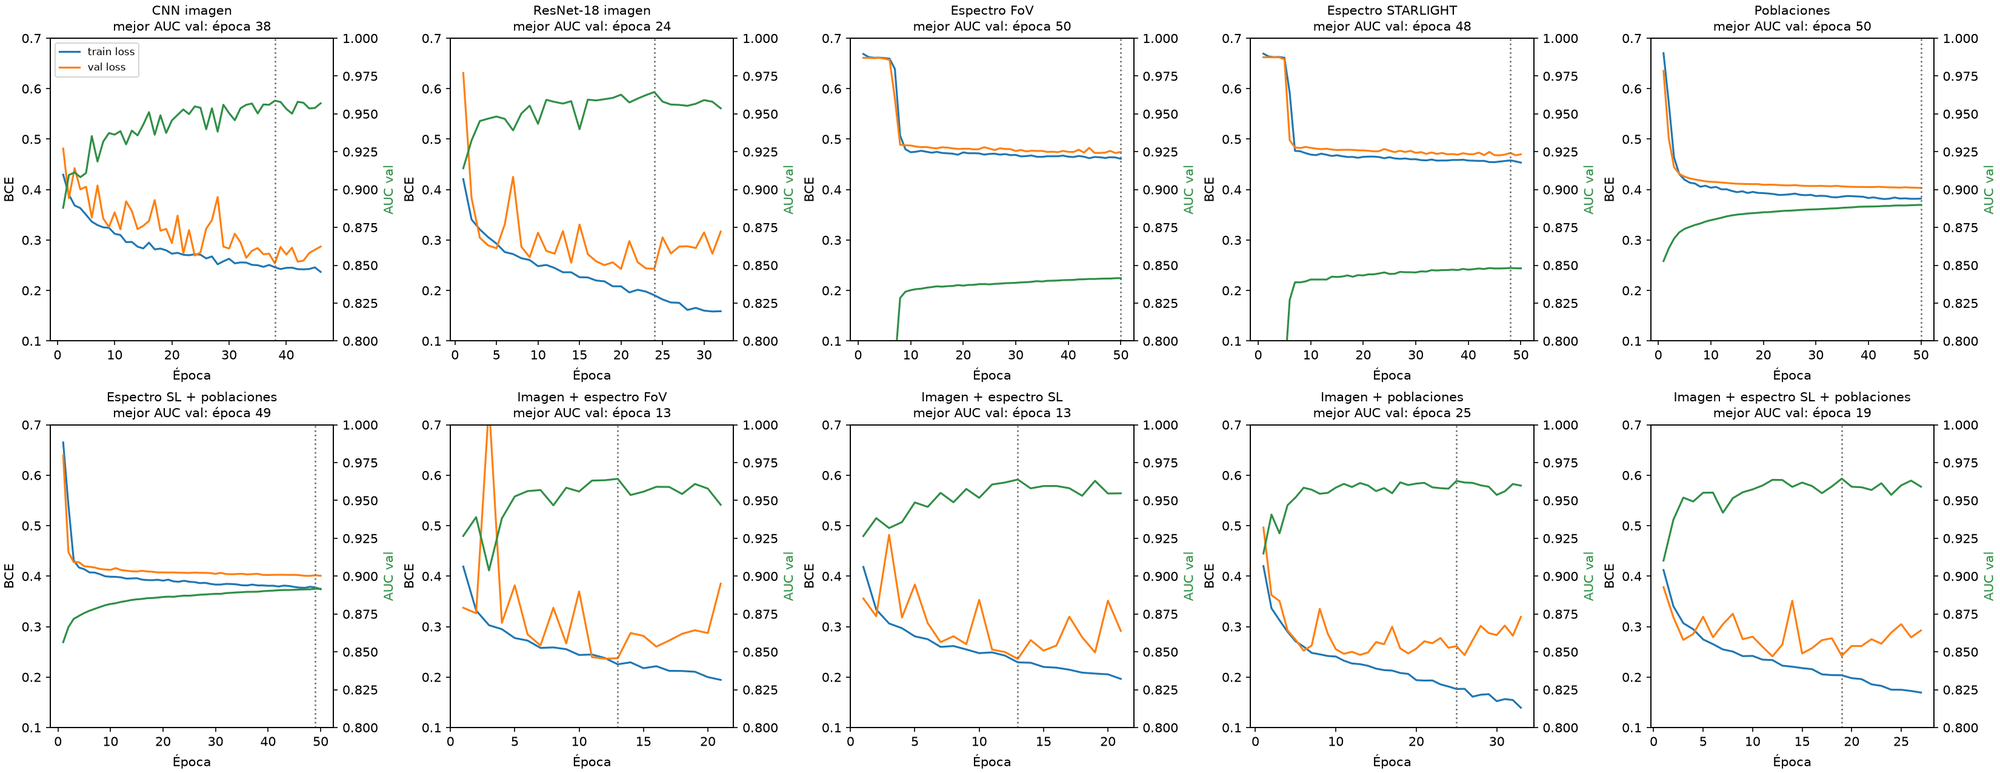
\includegraphics[width=0.65\textwidth]{curvas_entrenamiento.png}
    \caption{Curvas de entrenamiento.}
    \label{fig:crisp}
\end{figure}

\textbf{Modelos preentrenados}. 

Todos los encoders se entrenaron desde cero. 

\textbf{Compresión}

La \texttt{CNN} pequeña (1.2M parámetros) empata con \texttt{ResNet-18} (11M), lo que equivale a una compresión por diseño.

% ------------------------------------------------------------
\subsubsection{Fase 4: Evaluación}
% ------------------------------------------------------------

Comparación de modalidades en el conjunto de prueba: \texttt{ROC\-AUC} y \texttt{balanced accuracy} de cada experimento.

\begin{figure}[H]
    \centering
    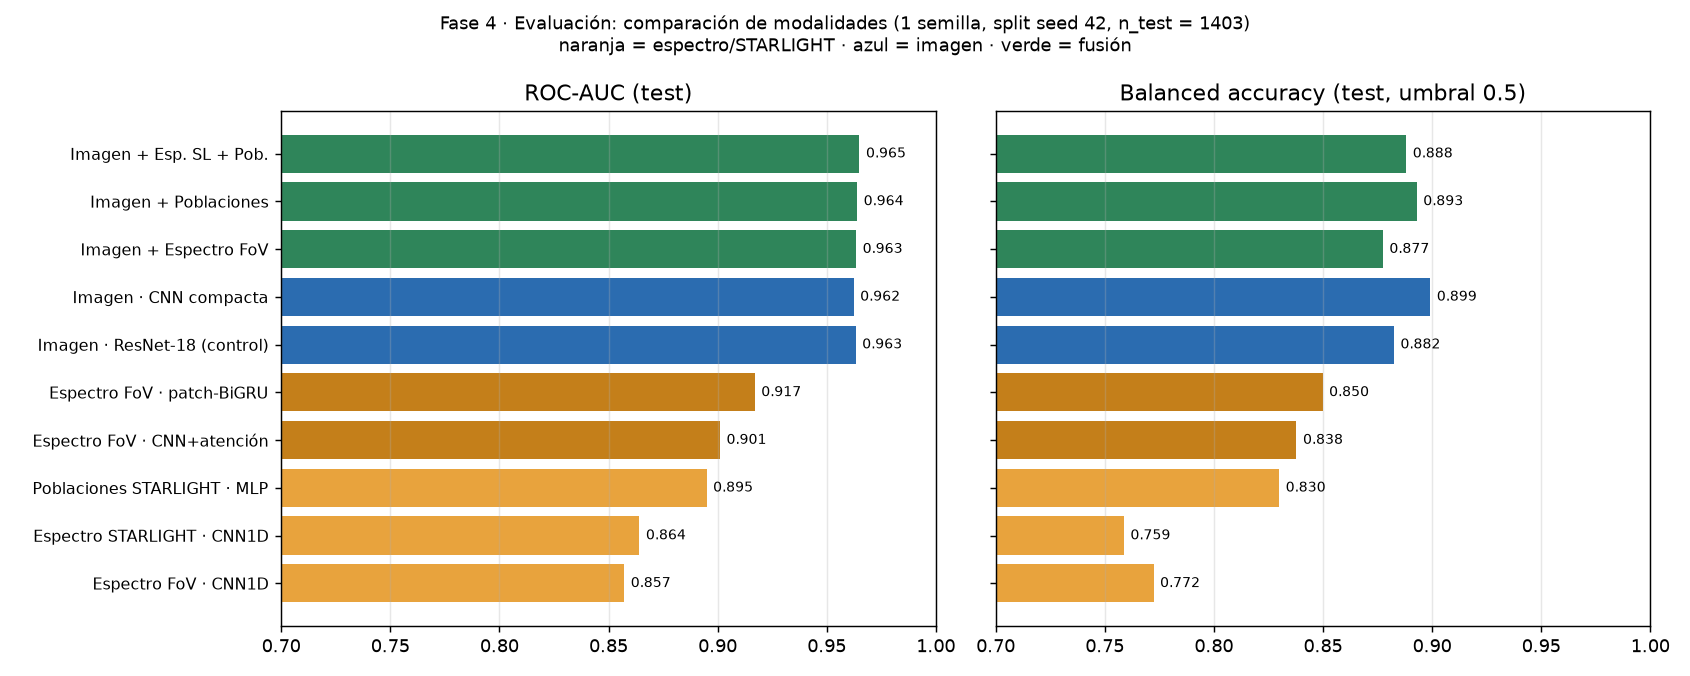
\includegraphics[width=0.65\textwidth]{fase4_comparacion_modalidades.png}
    \caption{Comparacion modalidades.}
    \label{fig:crisp}
\end{figure}

\textbf{Validar el desempeño}

\begin{figure}[H]
    \centering
    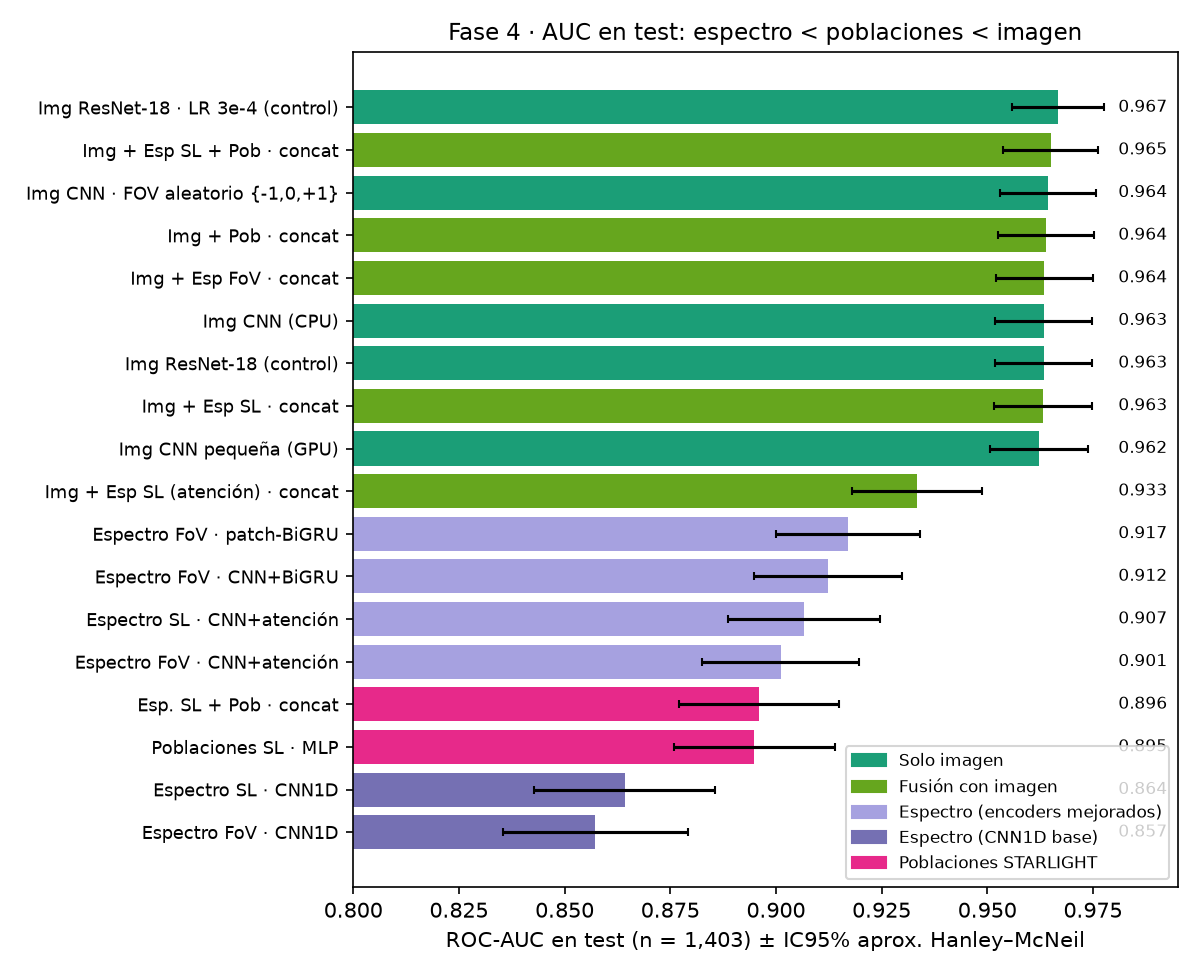
\includegraphics[width=0.65\textwidth]{fig2_auc_test.png}
    \caption{ROC-AUC en test de todos los experimentos.}
    \label{fig:crisp}
\end{figure}

\begin{table}[H]
\centering
\small
\begin{tabular}{|p{0.15\textwidth}|p{0.10\textwidth}|p{0.10\textwidth}|p{0.10\textwidth}|p{0.10\textwidth}|p{0.10\textwidth}|}
\hline
\textbf{Experimento} & \textbf{AUC} & \textbf{ACC} & \textbf{F1 macro} & \textbf{Rec. T}& \textbf{Rec. L} \\ \hline

Img ResNet-18 · LR 3e-4 &
0.9667 &
0.895 &
 &
0.909 &
0.887 \\ \hline

Img + Esp SL + Pob &
0.9650 &
0.890 &
0.884 &
0.883 &
0.894 \\ \hline

Img CNN · FOV aleatorio &
0.9643 &
0.900 &
0.895 &
0.900 &
0.901 \\ \hline

Img ResNet-18 (LR 1e-4) &
0.9633 &
0.888 &
0.881 &
0.860 &
0.905 \\ \hline

Img CNN (GPU) &
0.9623 &
0.901 &
0.895 &
0.892 &
0.906 \\ \hline

Img + Esp SL atención &
0.9334 &
0.862 &
 &
0.902 &
0.838 \\ \hline

Espectro FoV · patch-BiGRU &
0.9170 &
0.853 &
0.845 &
0.839 &
0.861 \\ \hline

Espectro SL · CNN + atención &
0.9066 &
0.842 &
0.833 &
0.812 &
0.859 \\ \hline

Poblaciones MLP &
0.8949 &
0.838 &
0.828 &
0.799 &
0.861 \\ \hline

Espectro FoV · CNN1D &
0.8572 &
0.795 &
0.777 &
0.682 &
0.863 \\ \hline

\end{tabular}
\caption{Comparación Modalidades}
\label{aplicacion}
\end{table}

\begin{table}[H]
\centering
\small
\begin{tabular}{|p{0.15\textwidth}|p{0.10\textwidth}|p{0.10\textwidth}|p{0.10\textwidth}|p{0.10\textwidth}|}
\hline
\textbf{Experimento} & \textbf{ROC-AUC} & \textbf{Balanced acc} & \textbf{Recall temprana} & \textbf{Recall tardía} \\ \hline

Espectro FoV · CNN1D &
0,857 &
0,772 &
0,682&
0,863 \\ \hline

Poblaciones STARLIGHT · MLP&
0,895 &
0,830 &
0,799 &
0,861 \\ \hline

Espectro FoV · patch-BiGRU &
0,917 &
0,850 &
0,839 &
0,861\\ \hline

Imagen · ResNet-18 (control) &
0,963 &
0,882&
0,860 &
0,905\\ \hline

Imagen + Espectro FoV &
0,963 &
0,877 &
0,837 &
0,918\\ \hline

Imagen + Esp. SL + Poblaciones &
0,965 &
0,888 &
0,883 &
0,894\\ \hline
\end{tabular}
\caption{Comparación Modalidades}
\label{aplicacion}
\end{table}

\textbf{Desempeño por segmentos.}

\begin{figure}[H]
    \centering
    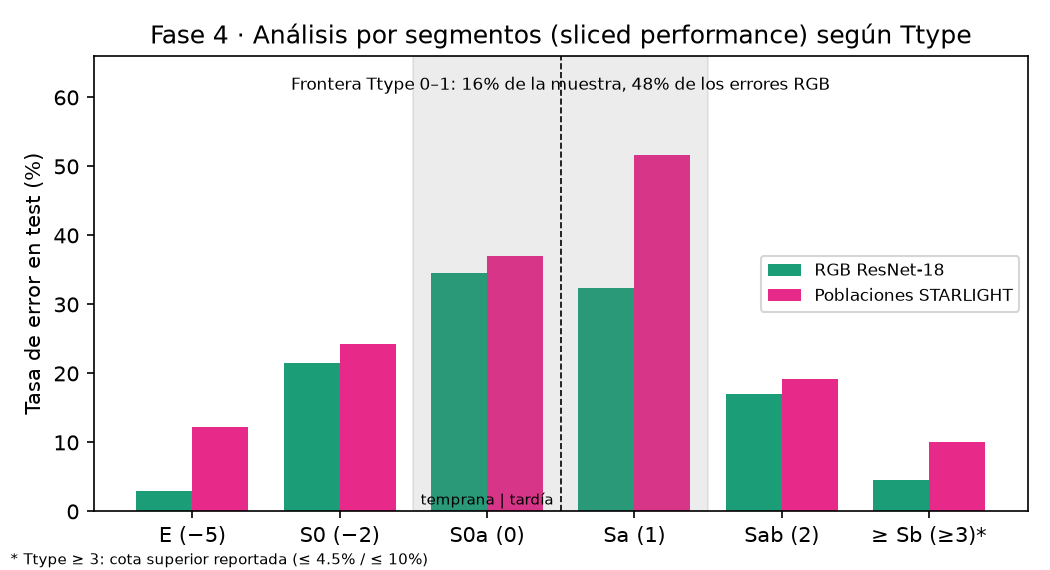
\includegraphics[width=0.65\textwidth]{fig3_error_por_ttype.png}
    \caption{Tasa de error según Ttype.}
    \label{fig:crisp}
\end{figure}

\begin{itemize}
    \item La frontera T-Type 0–1 es el 16\% de la muestra y concentra el 48\% de los errores RGB (33\% de error frente a 7\% en el resto).
    \item Las poblaciones casi no separan Sa de S0 (51.7\% de error en T-Type 1).
\end{itemize}

\textbf{Decisión y backtracking.}

El objetivo se cumple con imágenes (AUC$\sim$0.96, balanced accuracy$\sim$0.90). Los espectros contienen información complementaria: corrigen alrededor del 50\% de los errores RGB, y un oráculo llegaría a 0.946 de Accuracy. Pero las fusiones probadas todavía no la aprovechan, así que conviene volver a las fases 2 y 3 antes del despliegue.

\begin{figure}[H]
    \centering
    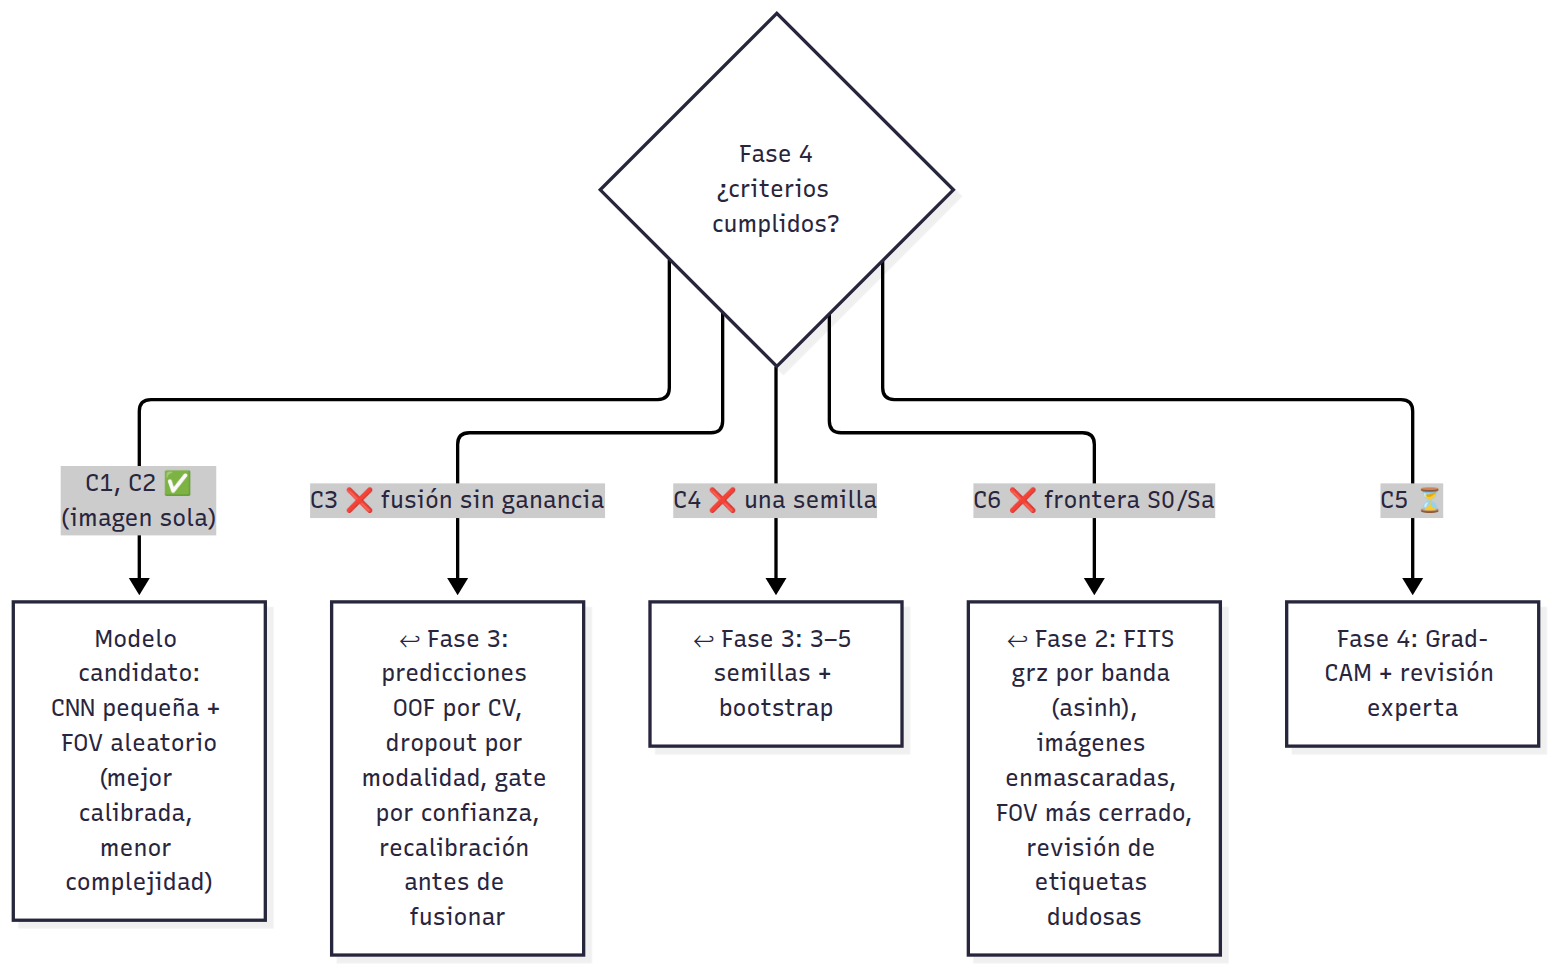
\includegraphics[width=0.65\textwidth]{diag6_backtracking.png}
    \caption{Decisión de la fase 4 y regreso a fases anteriores.}
    \label{fig:crisp}
\end{figure}

% ------------------------------------------------------------
\subsubsection{Concluciones}
% ------------------------------------------------------------

\begin{itemize}
    \item La combinación de imagen y espectro no mejora a la imagen sola. Todos los modelos con imagen rondan 0.96 de ROC-AUC y las diferencias entre ellos caen dentro del ruido.
    \item Errores en la frontera S0/Sa. Las galaxias con Ttype 0–1 son el 16\% de la muestra pero concentran el 48\% de los errores de las imágenes.
    \item Una sola semilla. Ningún experimento se repitió, así que no se pueden ordenar los modelos con imagen.
\end{itemize}

% ------------------------------------------------------------
\clearpage
\section{Anexos}
% ------------------------------------------------------------

% ------------------------------------------------------------
\subsection{Convenio}
% ------------------------------------------------------------

\includepdf[pages=-,scale=0.9,offset=0 0]{anexos/convenio.pdf}

% ------------------------------------------------------------
\subsection{Introducción del Proyecto Integrador}
% ------------------------------------------------------------

\includepdf[pages=-,scale=0.9,offset=0 0]{anexos/introduccion.pdf}

% ------------------------------------------------------------
\subsection{Revisión técnica de resultados}
% ------------------------------------------------------------
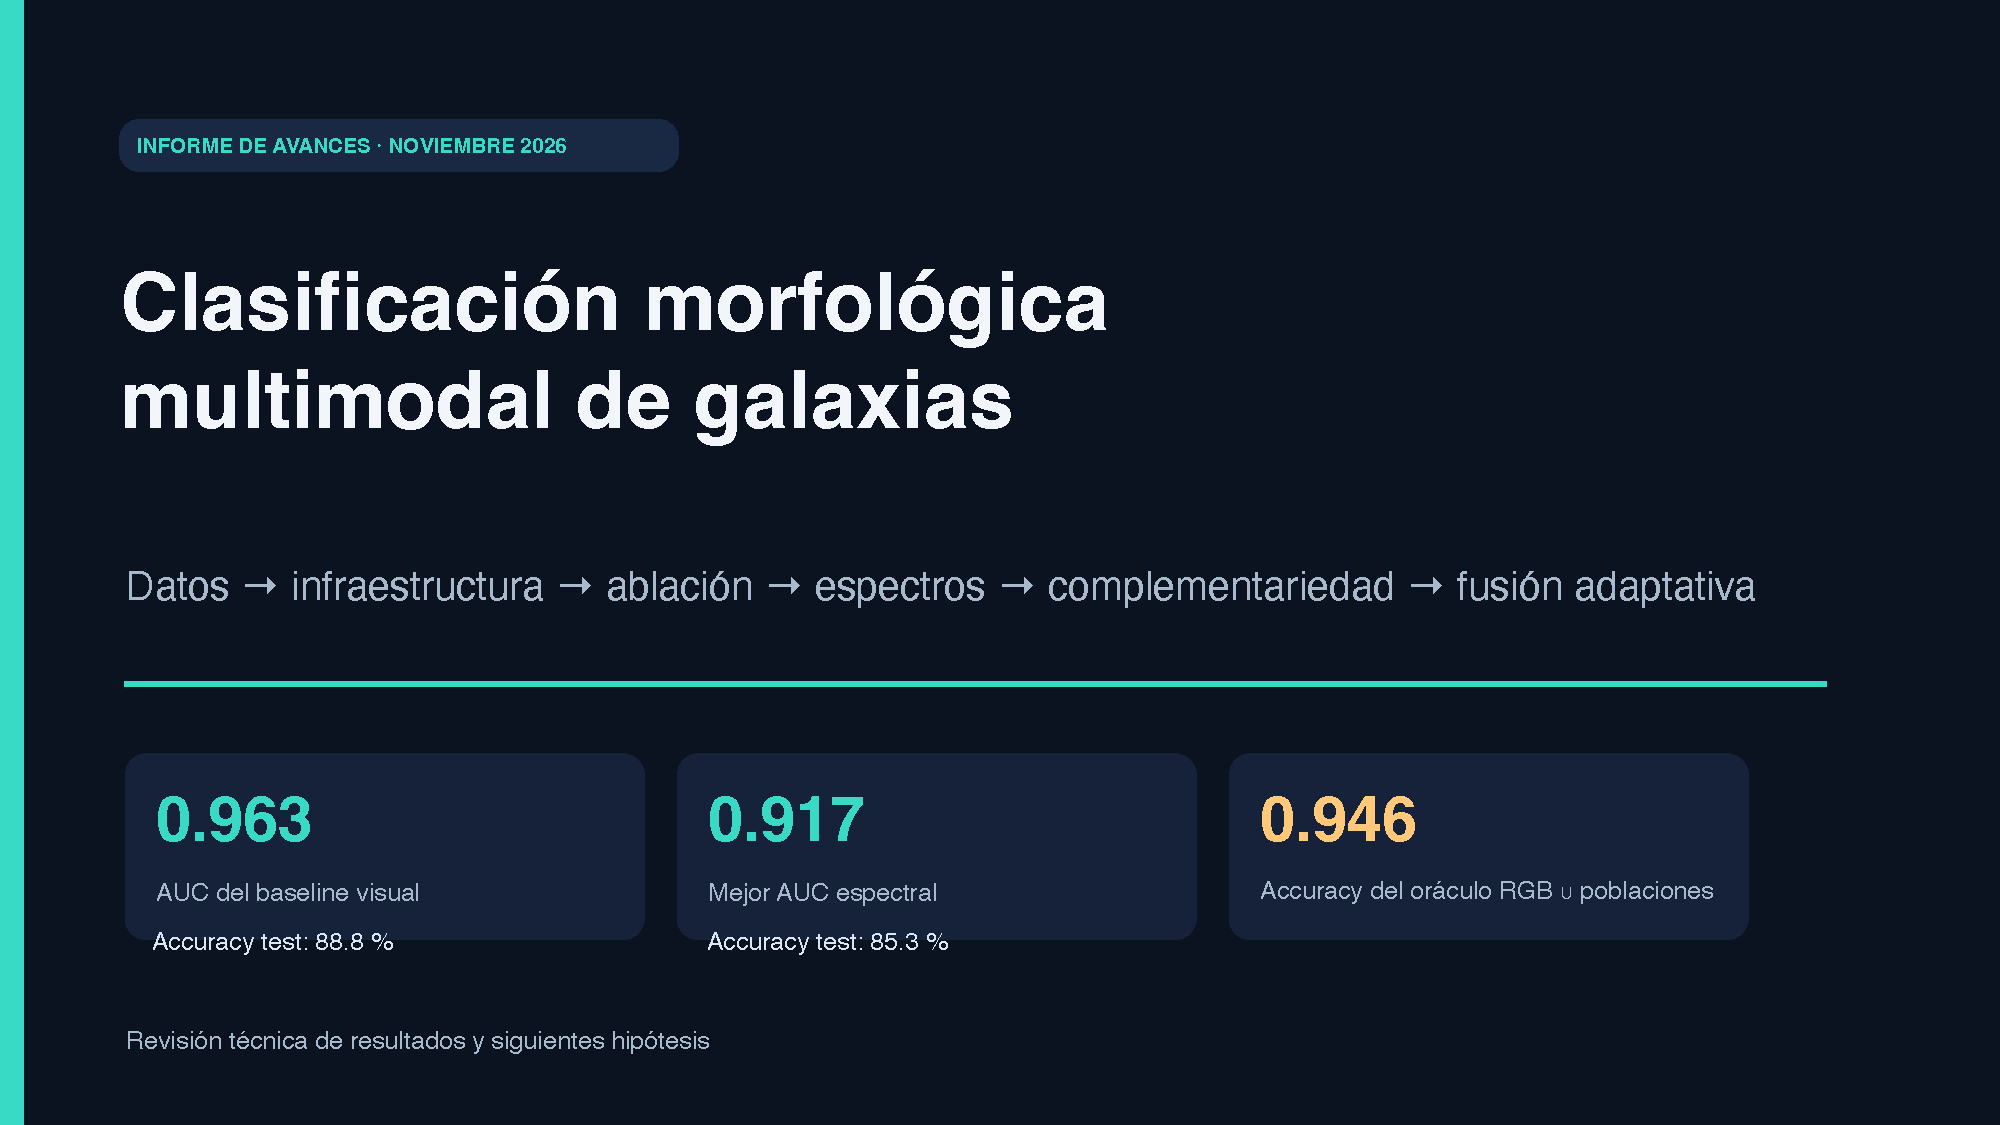
\includepdf[pages=-,scale=0.9,offset=0 0]{anexos/avances.pdf}

% ------------------------------------------------------------
\clearpage
\section{Referencias}
% ------------------------------------------------------------

\begin{itemize}

    \item Dey, A., Schlegel, D. J., Lang, D., Blum, R., Burleigh, K., Fan, X., Findlay, J. R., Finkbeiner, D., Herrera, D., Juneau, S., Landriau, M., Levi, M., McGreer, I., Meisner, A., Myers, A. D., Moustakas, J., Nugent, P., Patej, A., Schlafly, E. F., \& Walker, A. R. (2019). Overview of the DESI Legacy Imaging Surveys. \textit{The Astronomical Journal, 157}(5), 168. \url{https://doi.org/10.3847/1538-3881/ab089d}

    \item Karttunen, H., Kröger, P., Oja, H., Poutanen, M., \& Donner, K. J. (2007). \textit{Fundamental astronomy} (5th ed.). Springer. \url{https://doi.org/10.1007/978-3-540-34144-4}

    \item Studer, S., Bui, T. B., Drescher, C., Hanuschkin, A., Winkler, L., Peters, S., \& Müller, K.-R. (2021). Towards CRISP-ML(Q): A machine learning process model with quality assurance methodology. \textit{Machine Learning and Knowledge Extraction, 3}(2), 392--413. \url{https://doi.org/10.3390/make3020020}

    \item Vázquez-Mata, J. A., Hernández-Toledo, H. M., Avila-Reese, V., Cortes-Suárez, E., Aquino-Ortíz, E., \& Negrete, C. A. (2022). The SDSS-IV MaNGA visual morphology catalogue. \textit{Monthly Notices of the Royal Astronomical Society, 512}(2), 2222--2244.

    \item Hubble, E. P. (1926). Extragalactic nebulae. \textit{The Astrophysical Journal, 64}, 321--369. \url{https://doi.org/10.1086/143018}

    \item SeTIC-Ufsc. (n.d.). STARLIGHT Project. Universidade Federal De Santa Catarina. Fernandes, R. C. \url{https://minerva.ufsc.br/starlight/files/papers/Manual_StCv04.pdf}

    \item Fernandes, R. C., Gu, Q., Melnick, J., Terlevich, E., Terlevich, R., Kunth, D., Lacerda, R. R., \& Joguet, B. (2004). The star formation history of Seyfert 2 nuclei. \textit{Monthly Notices of the Royal Astronomical Society, 355}(1), 273–296. \url{https://doi.org/10.1111/j.1365-2966.2004.08321.x}

\end{itemize}

\end{document}
